\documentclass[]{book}
\usepackage{lmodern}
\usepackage{amssymb,amsmath}
\usepackage{ifxetex,ifluatex}
\usepackage{fixltx2e} % provides \textsubscript
\ifnum 0\ifxetex 1\fi\ifluatex 1\fi=0 % if pdftex
  \usepackage[T1]{fontenc}
  \usepackage[utf8]{inputenc}
\else % if luatex or xelatex
  \ifxetex
    \usepackage{mathspec}
  \else
    \usepackage{fontspec}
  \fi
  \defaultfontfeatures{Ligatures=TeX,Scale=MatchLowercase}
\fi
% use upquote if available, for straight quotes in verbatim environments
\IfFileExists{upquote.sty}{\usepackage{upquote}}{}
% use microtype if available
\IfFileExists{microtype.sty}{%
\usepackage{microtype}
\UseMicrotypeSet[protrusion]{basicmath} % disable protrusion for tt fonts
}{}
\usepackage{hyperref}
\hypersetup{unicode=true,
            pdftitle={Text Analysis with R},
            pdfauthor={Claudia Engel, Scott Bailey},
            pdfborder={0 0 0},
            breaklinks=true}
\urlstyle{same}  % don't use monospace font for urls
\usepackage{natbib}
\bibliographystyle{apalike}
\usepackage{color}
\usepackage{fancyvrb}
\newcommand{\VerbBar}{|}
\newcommand{\VERB}{\Verb[commandchars=\\\{\}]}
\DefineVerbatimEnvironment{Highlighting}{Verbatim}{commandchars=\\\{\}}
% Add ',fontsize=\small' for more characters per line
\usepackage{framed}
\definecolor{shadecolor}{RGB}{248,248,248}
\newenvironment{Shaded}{\begin{snugshade}}{\end{snugshade}}
\newcommand{\AlertTok}[1]{\textcolor[rgb]{0.94,0.16,0.16}{#1}}
\newcommand{\AnnotationTok}[1]{\textcolor[rgb]{0.56,0.35,0.01}{\textbf{\textit{#1}}}}
\newcommand{\AttributeTok}[1]{\textcolor[rgb]{0.77,0.63,0.00}{#1}}
\newcommand{\BaseNTok}[1]{\textcolor[rgb]{0.00,0.00,0.81}{#1}}
\newcommand{\BuiltInTok}[1]{#1}
\newcommand{\CharTok}[1]{\textcolor[rgb]{0.31,0.60,0.02}{#1}}
\newcommand{\CommentTok}[1]{\textcolor[rgb]{0.56,0.35,0.01}{\textit{#1}}}
\newcommand{\CommentVarTok}[1]{\textcolor[rgb]{0.56,0.35,0.01}{\textbf{\textit{#1}}}}
\newcommand{\ConstantTok}[1]{\textcolor[rgb]{0.00,0.00,0.00}{#1}}
\newcommand{\ControlFlowTok}[1]{\textcolor[rgb]{0.13,0.29,0.53}{\textbf{#1}}}
\newcommand{\DataTypeTok}[1]{\textcolor[rgb]{0.13,0.29,0.53}{#1}}
\newcommand{\DecValTok}[1]{\textcolor[rgb]{0.00,0.00,0.81}{#1}}
\newcommand{\DocumentationTok}[1]{\textcolor[rgb]{0.56,0.35,0.01}{\textbf{\textit{#1}}}}
\newcommand{\ErrorTok}[1]{\textcolor[rgb]{0.64,0.00,0.00}{\textbf{#1}}}
\newcommand{\ExtensionTok}[1]{#1}
\newcommand{\FloatTok}[1]{\textcolor[rgb]{0.00,0.00,0.81}{#1}}
\newcommand{\FunctionTok}[1]{\textcolor[rgb]{0.00,0.00,0.00}{#1}}
\newcommand{\ImportTok}[1]{#1}
\newcommand{\InformationTok}[1]{\textcolor[rgb]{0.56,0.35,0.01}{\textbf{\textit{#1}}}}
\newcommand{\KeywordTok}[1]{\textcolor[rgb]{0.13,0.29,0.53}{\textbf{#1}}}
\newcommand{\NormalTok}[1]{#1}
\newcommand{\OperatorTok}[1]{\textcolor[rgb]{0.81,0.36,0.00}{\textbf{#1}}}
\newcommand{\OtherTok}[1]{\textcolor[rgb]{0.56,0.35,0.01}{#1}}
\newcommand{\PreprocessorTok}[1]{\textcolor[rgb]{0.56,0.35,0.01}{\textit{#1}}}
\newcommand{\RegionMarkerTok}[1]{#1}
\newcommand{\SpecialCharTok}[1]{\textcolor[rgb]{0.00,0.00,0.00}{#1}}
\newcommand{\SpecialStringTok}[1]{\textcolor[rgb]{0.31,0.60,0.02}{#1}}
\newcommand{\StringTok}[1]{\textcolor[rgb]{0.31,0.60,0.02}{#1}}
\newcommand{\VariableTok}[1]{\textcolor[rgb]{0.00,0.00,0.00}{#1}}
\newcommand{\VerbatimStringTok}[1]{\textcolor[rgb]{0.31,0.60,0.02}{#1}}
\newcommand{\WarningTok}[1]{\textcolor[rgb]{0.56,0.35,0.01}{\textbf{\textit{#1}}}}
\usepackage{longtable,booktabs}
\usepackage{graphicx,grffile}
\makeatletter
\def\maxwidth{\ifdim\Gin@nat@width>\linewidth\linewidth\else\Gin@nat@width\fi}
\def\maxheight{\ifdim\Gin@nat@height>\textheight\textheight\else\Gin@nat@height\fi}
\makeatother
% Scale images if necessary, so that they will not overflow the page
% margins by default, and it is still possible to overwrite the defaults
% using explicit options in \includegraphics[width, height, ...]{}
\setkeys{Gin}{width=\maxwidth,height=\maxheight,keepaspectratio}
\IfFileExists{parskip.sty}{%
\usepackage{parskip}
}{% else
\setlength{\parindent}{0pt}
\setlength{\parskip}{6pt plus 2pt minus 1pt}
}
\setlength{\emergencystretch}{3em}  % prevent overfull lines
\providecommand{\tightlist}{%
  \setlength{\itemsep}{0pt}\setlength{\parskip}{0pt}}
\setcounter{secnumdepth}{5}
% Redefines (sub)paragraphs to behave more like sections
\ifx\paragraph\undefined\else
\let\oldparagraph\paragraph
\renewcommand{\paragraph}[1]{\oldparagraph{#1}\mbox{}}
\fi
\ifx\subparagraph\undefined\else
\let\oldsubparagraph\subparagraph
\renewcommand{\subparagraph}[1]{\oldsubparagraph{#1}\mbox{}}
\fi

%%% Use protect on footnotes to avoid problems with footnotes in titles
\let\rmarkdownfootnote\footnote%
\def\footnote{\protect\rmarkdownfootnote}

%%% Change title format to be more compact
\usepackage{titling}

% Create subtitle command for use in maketitle
\providecommand{\subtitle}[1]{
  \posttitle{
    \begin{center}\large#1\end{center}
    }
}

\setlength{\droptitle}{-2em}

  \title{Text Analysis with R}
    \pretitle{\vspace{\droptitle}\centering\huge}
  \posttitle{\par}
    \author{Claudia Engel, Scott Bailey}
    \preauthor{\centering\large\emph}
  \postauthor{\par}
      \predate{\centering\large\emph}
  \postdate{\par}
    \date{Last updated: July 02, 2019}

\usepackage{booktabs}
\usepackage{amsthm}
\makeatletter
\def\thm@space@setup{%
  \thm@preskip=8pt plus 2pt minus 4pt
  \thm@postskip=\thm@preskip
}
\makeatother

\begin{document}
\maketitle

{
\setcounter{tocdepth}{1}
\tableofcontents
}
\hypertarget{prerequisites}{%
\chapter*{Prerequisites}\label{prerequisites}}
\addcontentsline{toc}{chapter}{Prerequisites}

\begin{itemize}
\item
  You should have some \textbf{basic knowledge} of R, and be familiar with the topics covered in the \href{https://cengel.github.io/R-intro/}{Introduction to R}.
\item
  Have a \textbf{recent} version of \href{https://cran.r-project.org/}{R} and \href{https://www.rstudio.com/}{RStudio} installed.
\item
  Packages needed:

  \begin{itemize}
  \tightlist
  \item
    \texttt{tidyverse}
  \item
    \texttt{tidytext}
  \item
    \texttt{readtext}
  \item
    \texttt{sotu}
  \item
    \texttt{SnowballC}
  \item
    \texttt{widyr}
  \item
    \texttt{igraph}
  \item
    \texttt{ggraph}
  \item
    \texttt{tm}
  \end{itemize}
\end{itemize}

It is recommended that you not only intall, but also load the packages, to make sure the respective versions get along with your R version.

\hypertarget{references}{%
\section*{References}\label{references}}
\addcontentsline{toc}{section}{References}

Feinerer, I., Hornik, K., and Meyer, D. (2008). Text Mining Infrastructure in R. Journal of Statistical Software, 25(5), 1 - 54. \url{doi:http://dx.doi.org/10.18637/jss.v025.i05}

Gries, Stefan Thomas, 2009: \href{http://www.stgries.info/research/qclwr/qclwr.html}{Quantitative Corpus Linguistics with R: A Practical Introduction}. Routledge.

Silge, J and D. Robinson, 2017: \href{http://tidytextmining.com/}{Text Mining with R: A Tidy Approach}

Kasper Welbers, Wouter Van Atteveldt \& Kenneth Benoit (2017) Text Analysis in R, Communication Methods and Measures, 11:4, 245-265, DOI: 10.1080/19312458.2017.1387238

\href{https://CRAN.R-project.org/view=NaturalLanguageProcessing}{CRAN Task View: Natural Language Processing}

\hypertarget{textprep}{%
\chapter{Preparing Textual Data}\label{textprep}}

\begin{quote}
Learning Objectives

\begin{itemize}
\tightlist
\item
  read textual data into R using \texttt{readtext}
\item
  use \texttt{stringr} package to manipulate strings
\item
  use \texttt{tidytext} functions to tokenize texts and remove stopwords
\item
  use \texttt{SnowballC} to stem words
\end{itemize}
\end{quote}

\begin{center}\rule{0.5\linewidth}{\linethickness}\end{center}

We'll use several R packages in this section:

\begin{itemize}
\tightlist
\item
  \texttt{sotu} will provide the metadata and text of State of the Union speeches ranging from George Washington to Barack Obama.
\item
  \texttt{tidyverse} is a collection of R packages designed for data science, including \texttt{dplyr} with a set of verbs for common data manipulations and \texttt{ggplot2} for visualization.
\item
  \texttt{tidytext} provides specific functions for a ``tidy'' approach to working with textual data, where one row represents one ``token'' or meaningful unit of text, for example a word.
\item
  \texttt{readtext} provides a function well suited to reading textual data from a large number of formats into R, including metadata.
\end{itemize}

\begin{Shaded}
\begin{Highlighting}[]
\KeywordTok{library}\NormalTok{(sotu)}
\KeywordTok{library}\NormalTok{(tidyverse)}
\KeywordTok{library}\NormalTok{(tidytext)}
\KeywordTok{library}\NormalTok{(readtext)}
\end{Highlighting}
\end{Shaded}

\hypertarget{reading-text-into-r}{%
\section{Reading text into R}\label{reading-text-into-r}}

First, let's look at the data in the \texttt{sotu} package. The metadata and texts come separately. Below is what the metadata look like. Can you tell how many speeches we have?

\begin{Shaded}
\begin{Highlighting}[]
\CommentTok{# Let's take a quick look at the state of the union metadata}
\KeywordTok{str}\NormalTok{(sotu_meta)}
\end{Highlighting}
\end{Shaded}

\begin{verbatim}
#> Classes 'tbl_df', 'tbl' and 'data.frame':    236 obs. of  5 variables:
#>  $ president   : chr  "George Washington" "George Washington" "George Washington" "George Washington" ...
#>  $ year        : int  1790 1790 1791 1792 1793 1794 1795 1796 1797 1798 ...
#>  $ years_active: chr  "1789-1793" "1789-1793" "1789-1793" "1789-1793" ...
#>  $ party       : chr  "Nonpartisan" "Nonpartisan" "Nonpartisan" "Nonpartisan" ...
#>  $ sotu_type   : chr  "speech" "speech" "speech" "speech" ...
\end{verbatim}

In order to work with the speech texts and to later practice reading text files from disk we're going to use a function \texttt{sotu\_dir} to write the texts out. This function by default writes to a temporary directory with one speech in each file. It returns a character vector where each element is the name of the path to the individual speech file. We save this vector into the \texttt{file\_paths} variable.

\begin{Shaded}
\begin{Highlighting}[]
\CommentTok{# sotu_dir writes the text files to disk in a temporary dir, }
\CommentTok{# but you could specific where you want them.}
\NormalTok{file_paths <-}\StringTok{ }\KeywordTok{sotu_dir}\NormalTok{()}
\KeywordTok{head}\NormalTok{(file_paths)}
\end{Highlighting}
\end{Shaded}

\begin{verbatim}
#> [1] "/var/folders/5y/9x92pjcx2xd2h7qxqx39vpmc0000gn/T//RtmpVz6bBx/file304733ab7d52/george-washington-1790a.txt"
#> [2] "/var/folders/5y/9x92pjcx2xd2h7qxqx39vpmc0000gn/T//RtmpVz6bBx/file304733ab7d52/george-washington-1790b.txt"
#> [3] "/var/folders/5y/9x92pjcx2xd2h7qxqx39vpmc0000gn/T//RtmpVz6bBx/file304733ab7d52/george-washington-1791.txt" 
#> [4] "/var/folders/5y/9x92pjcx2xd2h7qxqx39vpmc0000gn/T//RtmpVz6bBx/file304733ab7d52/george-washington-1792.txt" 
#> [5] "/var/folders/5y/9x92pjcx2xd2h7qxqx39vpmc0000gn/T//RtmpVz6bBx/file304733ab7d52/george-washington-1793.txt" 
#> [6] "/var/folders/5y/9x92pjcx2xd2h7qxqx39vpmc0000gn/T//RtmpVz6bBx/file304733ab7d52/george-washington-1794.txt"
\end{verbatim}

Now that we have the files on disk and a vector of filepaths, we can pass this vector directly into \texttt{readtext} to read the texts into a new variable.

\begin{Shaded}
\begin{Highlighting}[]
\CommentTok{# let's read in the files with readtext}
\NormalTok{sotu_texts <-}\StringTok{ }\KeywordTok{readtext}\NormalTok{(file_paths)}
\KeywordTok{head}\NormalTok{(sotu_texts)}
\end{Highlighting}
\end{Shaded}

\begin{verbatim}
#> readtext object consisting of 6 documents and 0 docvars.
#> # Description: df[,2] [6 x 2]
#>   doc_id                   text                 
#> * <chr>                    <chr>                
#> 1 abraham-lincoln-1861.txt "\"\n\n Fellow-\"..."
#> 2 abraham-lincoln-1862.txt "\"\n\n Fellow-\"..."
#> 3 abraham-lincoln-1863.txt "\"\n\n Fellow-\"..."
#> 4 abraham-lincoln-1864.txt "\"\n\n Fellow-\"..."
#> 5 andrew-jackson-1829.txt  "\"\n\n Fellow \"..."
#> 6 andrew-jackson-1830.txt  "\"\n\n Fellow \"..."
\end{verbatim}

To work with a single tabular dataset, we combine the text and metadata into a single tibble. You can see that our \texttt{sotu\_texts} are organized by alphabetical order, so first we'll need to sort our metadata to match.

\begin{Shaded}
\begin{Highlighting}[]
\NormalTok{sotu_whole <-}\StringTok{ }
\StringTok{  }\NormalTok{sotu_meta }\OperatorTok\StringTok{  }
\StringTok{  }\KeywordTok{arrange}\NormalTok{(president) }\OperatorTok\StringTok{ }\CommentTok{# sort metadata}
\StringTok{  }\KeywordTok{bind_cols}\NormalTok{(sotu_texts) }\CommentTok{# combine with texts}

\KeywordTok{glimpse}\NormalTok{(sotu_whole)}
\end{Highlighting}
\end{Shaded}

\begin{verbatim}
#> Observations: 236
#> Variables: 7
#> $ president    <chr> "Abraham Lincoln", "Abraham Lincoln", "Abraham Li...
#> $ year         <int> 1861, 1862, 1863, 1864, 1829, 1830, 1831, 1832, 1...
#> $ years_active <chr> "1861-1865", "1861-1865", "1861-1865", "1861-1865...
#> $ party        <chr> "Republican", "Republican", "Republican", "Republ...
#> $ sotu_type    <chr> "written", "written", "written", "written", "writ...
#> $ doc_id       <chr> "abraham-lincoln-1861.txt", "abraham-lincoln-1862...
#> $ text         <chr> "\n\n Fellow-Citizens of the Senate and House of ...
\end{verbatim}

Now that we have our data, we need to think about cleaning it. Depending on the quality of your data, you might need to explicitly replace certain characters or words, remove urls or types of numbers, such as phone numbers, or otherwise clean up misspellings or errors. There are several ways to handle this sort of cleaning, we'll show a few examples for string manipulation and replacement.

\hypertarget{string-operations}{%
\section{String operations}\label{string-operations}}

R has many functions available to manipulate strings including functions like \texttt{grep} and \texttt{paste}, which come with the R base install.

Here we will here take a look at the \texttt{stringr} package, which is part of the \texttt{tidyverse}. Under the hood it wraps a lot of the functions from the \texttt{stringi} package which is perhaps one of the most comprehensive string manipulation packages.

Below are examples for a few functions that might be useful.

\texttt{str\_count} takes a characer vector as input and by default counts the number of pattern matches in a string.

How man times does the word ``citizen'' appear in each of the speeches?

\begin{Shaded}
\begin{Highlighting}[]
\NormalTok{sotu_whole }\OperatorTok\StringTok{ }
\StringTok{  }\KeywordTok{pull}\NormalTok{(text) }\OperatorTok\StringTok{ }\CommentTok{# extract texts vector}
\StringTok{  }\KeywordTok{str_count}\NormalTok{(}\StringTok{"citizen"}\NormalTok{)}
\end{Highlighting}
\end{Shaded}

\begin{verbatim}
#>   [1]  9  7 15  3 19 14 23 19 14 25 10  9 11 10 11 12  3  6  3  6  7  3  2
#>  [24]  8 14 13 17 15 13  3  5  6  9  7 14  9 20 17 14 17 23  1  8  6  0  6
#>  [47]  4  3  3  1  2  2  6  1  3  2  1  1  6  2  3 12 17 17 29  2  3  4  1
#>  [70]  5  9  9  6  7  9 11 10  2  4  2  6  4 10  3  5  0  8  6 43 42  5 37
#>  [93] 19 16 21 16  7  5 10  6  8  4  2 11  9  3  4  1 13 41 30 35 29 42 34
#> [116] 15  3  3  4  4  4  2  3  5  7  8  6  3  6  1  7  9  4  9  3 15  4 24
#> [139] 25  8  2  3  1  2  7  6 10  6 11  8 13 13 11  9  5  3  2  6  2  2 14
#> [162] 27 17 13 13 16 14  0  0  0  8  2 10  2  4  3  4  5  2  3  0 15 17 27
#> [185] 20 13  1 19 27 31 28 18 10 10  6  7  3  9  6  5  8 15 16 17 22 20 28
#> [208] 29 22  4  5  9 10 10 27  1  2 21 12 10  9  3  8 20 12 26 13  4  2  8
#> [231]  0  0  0  0  0 11
\end{verbatim}

It is possible to use regular expressions, for example, this is how we would check how many times either ``citizen'' or ``Citizen'' appear in each of the speeches:

\begin{Shaded}
\begin{Highlighting}[]
\NormalTok{sotu_whole }\OperatorTok\StringTok{ }
\StringTok{  }\KeywordTok{pull}\NormalTok{(text) }\OperatorTok\StringTok{ }\CommentTok{# extract texts vector}
\StringTok{  }\KeywordTok{str_count}\NormalTok{(}\StringTok{"[C|c]itizen"}\NormalTok{)}
\end{Highlighting}
\end{Shaded}

\begin{verbatim}
#>   [1] 10  8 16  4 20 15 24 20 15 26 11 10 12 11 12 13  3  6  3  6  7  6  2
#>  [24]  8 14 13 17 15 13  3  5  6  9  7 14  9 20 17 14 17 23  2  8  6  0  6
#>  [47]  4  3  3  1  2  2  6  1  3  2  1  1  6  2  3 13 18 18 30  2  3  4  1
#>  [70]  5  9 10  6  7  9 11 10  3  5  3  7  5 11  4  6  0  8  6 43 42  5 37
#>  [93] 19 16 21 16  7  5 10  6  8  4  2 11  9  3  4  1 15 42 31 36 30 43 35
#> [116] 16  4  4  5  5  5  3  4  6  8  9  7  4  7  2  8 10  4  9  3 15  4 24
#> [139] 25  8  2  3  1  2  7  6 11  7 12  9 13 14 11  9  5  3  2  6  2  2 15
#> [162] 28 18 14 15 17 15  0  0  0  8  2 10  2  4  3  4  5  2  3  0 16 18 28
#> [185] 21 13  1 19 27 31 28 18 10 11  6  7  3  9  6  5  8 15 16 17 22 20 28
#> [208] 29 22  4  5  9 10 10 27  1  2 22 12 11  9  3  8 20 12 26 13  4  2  8
#> [231]  0  0  0  0  0 12
\end{verbatim}

When used with the \texttt{boundary} argument \texttt{str\_count} can count different entities like ``character'', ``line\_break'', ``sentence'', or ``word''. Here we add a new column to the dataframe indicating how many words are there in each speech:

\begin{Shaded}
\begin{Highlighting}[]
\NormalTok{sotu_whole }\OperatorTok\StringTok{ }
\StringTok{  }\KeywordTok{mutate}\NormalTok{(}\DataTypeTok{n_words =} \KeywordTok{str_count}\NormalTok{(text, }\KeywordTok{boundary}\NormalTok{(}\StringTok{"word"}\NormalTok{))) }
\end{Highlighting}
\end{Shaded}

\begin{verbatim}
#> # A tibble: 236 x 8
#>    president   year years_active party  sotu_type doc_id  text      n_words
#>    <chr>      <int> <chr>        <chr>  <chr>     <chr>   <chr>       <int>
#>  1 Abraham L~  1861 1861-1865    Repub~ written   abraha~ "\n\n Fe~    6998
#>  2 Abraham L~  1862 1861-1865    Repub~ written   abraha~ "\n\n Fe~    8410
#>  3 Abraham L~  1863 1861-1865    Repub~ written   abraha~ "\n\n Fe~    6132
#>  4 Abraham L~  1864 1861-1865    Repub~ written   abraha~ "\n\n Fe~    5975
#>  5 Andrew Ja~  1829 1829-1833    Democ~ written   andrew~ "\n\n Fe~   10547
#>  6 Andrew Ja~  1830 1829-1833    Democ~ written   andrew~ "\n\n Fe~   15109
#>  7 Andrew Ja~  1831 1829-1833    Democ~ written   andrew~ "\n\n Fe~    7198
#>  8 Andrew Ja~  1832 1829-1833    Democ~ written   andrew~ "\n\n Fe~    7887
#>  9 Andrew Ja~  1833 1833-1837    Democ~ written   andrew~ "\n\n Fe~    7912
#> 10 Andrew Ja~  1834 1833-1837    Democ~ written   andrew~ "\n\n Fe~   13472
#> # ... with 226 more rows
\end{verbatim}

\begin{quote}
\begin{quote}
\begin{quote}
CHALLENGE: Use the code above and add another column \texttt{n\_sentences} where you calculate the number of sentences per speech. Then create a third column \texttt{avg\_word\_per\_sentence}, where you calculate the number of words per sentence for each speech. Finally use \texttt{filter} to find which speech has shortest/longest average sentences length and what is the avderage length.
\end{quote}
\end{quote}
\end{quote}

\texttt{str\_detect} also looks for patterns, but instead of counts it returns a logical vector (TRUE/FALSE) indiciating if the pattern is or is not found. So we typically want to use it with the \texttt{filter} ``verb'' from \texttt{dplyr}.

What are the names of the documents where the words ``citizen'' and ``Citizen'' do \textbf{not} occur?

\begin{Shaded}
\begin{Highlighting}[]
\NormalTok{sotu_whole }\OperatorTok\StringTok{ }
\StringTok{  }\KeywordTok{filter}\NormalTok{(}\OperatorTok{!}\KeywordTok{str_detect}\NormalTok{(text, }\StringTok{"[C|c]itizen"}\NormalTok{)) }\OperatorTok\StringTok{ }
\StringTok{  }\KeywordTok{select}\NormalTok{(doc_id) }
\end{Highlighting}
\end{Shaded}

\begin{verbatim}
#> # A tibble: 11 x 1
#>    doc_id                      
#>    <chr>                       
#>  1 dwight-d-eisenhower-1958.txt
#>  2 gerald-r-ford-1975.txt      
#>  3 richard-m-nixon-1970.txt    
#>  4 richard-m-nixon-1971.txt    
#>  5 richard-m-nixon-1972a.txt   
#>  6 ronald-reagan-1988.txt      
#>  7 woodrow-wilson-1916.txt     
#>  8 woodrow-wilson-1917.txt     
#>  9 woodrow-wilson-1918.txt     
#> 10 woodrow-wilson-1919.txt     
#> 11 woodrow-wilson-1920.txt
\end{verbatim}

The \texttt{word} function extracts specific words from a character vector of words. By default it returns the first word. If for example we wanted to extract the first 5 words of each speech by Woodrow Wilson we provide the \texttt{end} argument like this:

\begin{Shaded}
\begin{Highlighting}[]
\NormalTok{sotu_whole }\OperatorTok\StringTok{ }
\StringTok{  }\KeywordTok{filter}\NormalTok{(president }\OperatorTok{==}\StringTok{ "Woodrow Wilson"}\NormalTok{) }\OperatorTok\StringTok{  }\CommentTok{# sample a few speeches as demo}
\StringTok{  }\KeywordTok{pull}\NormalTok{(text) }\OperatorTok\StringTok{ }\CommentTok{# extract character vector}
\StringTok{  }\KeywordTok{word}\NormalTok{(}\DataTypeTok{end =} \DecValTok{5}\NormalTok{) }\CommentTok{# end = 5 to extract words 1 - 5.}
\end{Highlighting}
\end{Shaded}

\begin{verbatim}
#> [1] "\n\nGentlemen of the Congress:\n\nIn pursuance"
#> [2] "\n\nGENTLEMEN OF THE CONGRESS: \n\nThe"        
#> [3] "GENTLEMEN OF THE CONGRESS: \n\nSince"          
#> [4] "\n\nGENTLEMEN OF THE CONGRESS: \n\nIn"         
#> [5] "Gentlemen of the Congress:\n\nEight months"    
#> [6] "\n\nGENTLEMEN OF THE CONGRESS: \n\nThe"        
#> [7] "\n\nTO THE SENATE AND HOUSE"                   
#> [8] "\n\nGENTLEMEN OF THE CONGRESS:\n\nWhen I"
\end{verbatim}

To clean this up a little we will first remove the newline characters (\texttt{\textbackslash{}n}). We use the \texttt{str\_replace\_all} function to replace all the ocurrences of the \texttt{\textbackslash{}n} pattern with a white space \texttt{"\ "}. We need to add the escape character \texttt{\textbackslash{}} in front of our pattern to be replaced so the backslash before the \texttt{n} is interpreted correctly.

\begin{Shaded}
\begin{Highlighting}[]
\NormalTok{sotu_whole }\OperatorTok\StringTok{ }
\StringTok{  }\KeywordTok{filter}\NormalTok{(president }\OperatorTok{==}\StringTok{ "Woodrow Wilson"}\NormalTok{) }\OperatorTok\StringTok{  }
\StringTok{  }\KeywordTok{pull}\NormalTok{(text) }\OperatorTok
\StringTok{  }\KeywordTok{str_replace_all}\NormalTok{(}\StringTok{"}\CharTok{\textbackslash{}\textbackslash{}}\StringTok{n"}\NormalTok{, }\StringTok{" "}\NormalTok{) }\OperatorTok\StringTok{ }\CommentTok{# replace newline}
\StringTok{  }\KeywordTok{word}\NormalTok{(}\DataTypeTok{end =} \DecValTok{5}\NormalTok{) }
\end{Highlighting}
\end{Shaded}

\begin{verbatim}
#> [1] "  Gentlemen of the"          "  GENTLEMEN OF THE"         
#> [3] "GENTLEMEN OF THE CONGRESS: " "  GENTLEMEN OF THE"         
#> [5] "Gentlemen of the Congress: " "  GENTLEMEN OF THE"         
#> [7] "  TO THE SENATE"             "  GENTLEMEN OF THE"
\end{verbatim}

This looks better, but we still have a problem to extract exactly 5 words because of the whitespaces. So let's get rid of any whitespaces before and also of repeated whitespaces within the string with the convenient \texttt{str\_squish} function.

\begin{Shaded}
\begin{Highlighting}[]
\NormalTok{sotu_whole }\OperatorTok\StringTok{ }
\StringTok{  }\KeywordTok{filter}\NormalTok{(president }\OperatorTok{==}\StringTok{ "Woodrow Wilson"}\NormalTok{) }\OperatorTok\StringTok{  }
\StringTok{  }\KeywordTok{pull}\NormalTok{(text) }\OperatorTok
\StringTok{  }\KeywordTok{str_replace_all}\NormalTok{(}\StringTok{"}\CharTok{\textbackslash{}\textbackslash{}}\StringTok{n"}\NormalTok{, }\StringTok{" "}\NormalTok{) }\OperatorTok\StringTok{ }
\StringTok{  }\KeywordTok{str_squish}\NormalTok{() }\OperatorTok\StringTok{  }\CommentTok{# remove whitespaces}
\StringTok{  }\KeywordTok{word}\NormalTok{(}\DataTypeTok{end =} \DecValTok{5}\NormalTok{) }
\end{Highlighting}
\end{Shaded}

\begin{verbatim}
#> [1] "Gentlemen of the Congress: In"    "GENTLEMEN OF THE CONGRESS: The"  
#> [3] "GENTLEMEN OF THE CONGRESS: Since" "GENTLEMEN OF THE CONGRESS: In"   
#> [5] "Gentlemen of the Congress: Eight" "GENTLEMEN OF THE CONGRESS: The"  
#> [7] "TO THE SENATE AND HOUSE"          "GENTLEMEN OF THE CONGRESS: When"
\end{verbatim}

(For spell checks take a look at \url{https://CRAN.R-project.org/package=spelling} or \url{https://CRAN.R-project.org/package=hunspell})

\hypertarget{tokenize-lowercase}{%
\section{Tokenize, lowercase}\label{tokenize-lowercase}}

A very common part of preparing your text for analysis involves tokenization. Currently our data contains in each each row a single text with metdata, so the entire speech text is the unit of observation. When we tokenize we break down the text into ``tokens'' (most commonly single words), so each row contains a single word with its metadata as unit of observation.

\texttt{tidytext} provides a function \texttt{unnest\_tokens} to convert our speech table into one that is tokenized. It takes three arguments:

\begin{itemize}
\tightlist
\item
  a tibble or data frame which contains the text;
\item
  the name of the newly created column that will contain the tokens;
\item
  the name of the column within the data frame which contains the text to be tokenized.
\end{itemize}

In the example below we name the new column to hold the tokens \texttt{word}. Remember that the column that holds the speech text is called \texttt{text}.

\begin{Shaded}
\begin{Highlighting}[]
\NormalTok{tidy_sotu <-}\StringTok{ }\NormalTok{sotu_whole }\OperatorTok
\StringTok{  }\KeywordTok{unnest_tokens}\NormalTok{(word, text)}

\NormalTok{tidy_sotu}
\end{Highlighting}
\end{Shaded}

\begin{verbatim}
#> # A tibble: 1,965,212 x 7
#>    president     year years_active party   sotu_type doc_id        word    
#>    <chr>        <int> <chr>        <chr>   <chr>     <chr>         <chr>   
#>  1 Abraham Lin~  1861 1861-1865    Republ~ written   abraham-linc~ fellow  
#>  2 Abraham Lin~  1861 1861-1865    Republ~ written   abraham-linc~ citizens
#>  3 Abraham Lin~  1861 1861-1865    Republ~ written   abraham-linc~ of      
#>  4 Abraham Lin~  1861 1861-1865    Republ~ written   abraham-linc~ the     
#>  5 Abraham Lin~  1861 1861-1865    Republ~ written   abraham-linc~ senate  
#>  6 Abraham Lin~  1861 1861-1865    Republ~ written   abraham-linc~ and     
#>  7 Abraham Lin~  1861 1861-1865    Republ~ written   abraham-linc~ house   
#>  8 Abraham Lin~  1861 1861-1865    Republ~ written   abraham-linc~ of      
#>  9 Abraham Lin~  1861 1861-1865    Republ~ written   abraham-linc~ represe~
#> 10 Abraham Lin~  1861 1861-1865    Republ~ written   abraham-linc~ in      
#> # ... with 1,965,202 more rows
\end{verbatim}

Note that the \texttt{unnest\_tokens} function didn't just tokenize our texts at the word level. It also lowercased each word and stripped off the punctuation. We can tell it not to do this, by adding the following parameters:

\begin{Shaded}
\begin{Highlighting}[]
\CommentTok{# Word tokenization with punctuation and no lowercasing}
\NormalTok{sotu_whole }\OperatorTok
\StringTok{  }\KeywordTok{unnest_tokens}\NormalTok{(word, text, }\DataTypeTok{to_lower =} \OtherTok{FALSE}\NormalTok{, }\DataTypeTok{strip_punct =} \OtherTok{FALSE}\NormalTok{)}
\end{Highlighting}
\end{Shaded}

\begin{verbatim}
#> # A tibble: 2,157,777 x 7
#>    president     year years_active party   sotu_type doc_id        word    
#>    <chr>        <int> <chr>        <chr>   <chr>     <chr>         <chr>   
#>  1 Abraham Lin~  1861 1861-1865    Republ~ written   abraham-linc~ Fellow  
#>  2 Abraham Lin~  1861 1861-1865    Republ~ written   abraham-linc~ -       
#>  3 Abraham Lin~  1861 1861-1865    Republ~ written   abraham-linc~ Citizens
#>  4 Abraham Lin~  1861 1861-1865    Republ~ written   abraham-linc~ of      
#>  5 Abraham Lin~  1861 1861-1865    Republ~ written   abraham-linc~ the     
#>  6 Abraham Lin~  1861 1861-1865    Republ~ written   abraham-linc~ Senate  
#>  7 Abraham Lin~  1861 1861-1865    Republ~ written   abraham-linc~ and     
#>  8 Abraham Lin~  1861 1861-1865    Republ~ written   abraham-linc~ House   
#>  9 Abraham Lin~  1861 1861-1865    Republ~ written   abraham-linc~ of      
#> 10 Abraham Lin~  1861 1861-1865    Republ~ written   abraham-linc~ Represe~
#> # ... with 2,157,767 more rows
\end{verbatim}

We can also tokenize the text at the level of ngrams or sentences, if those are the best units of analysis for our work.

\begin{Shaded}
\begin{Highlighting}[]
\CommentTok{# Sentence tokenization}
\NormalTok{sotu_whole }\OperatorTok
\StringTok{  }\KeywordTok{unnest_tokens}\NormalTok{(sentence, text, }\DataTypeTok{token =} \StringTok{"sentences"}\NormalTok{, }\DataTypeTok{to_lower =} \OtherTok{FALSE}\NormalTok{) }\OperatorTok\StringTok{ }
\StringTok{  }\KeywordTok{select}\NormalTok{(sentence)}
\end{Highlighting}
\end{Shaded}

\begin{verbatim}
#> # A tibble: 69,158 x 1
#>    sentence                                                                
#>    <chr>                                                                   
#>  1 Fellow-Citizens of the Senate and House of Representatives:   In the mi~
#>  2 You will not be surprised to learn that in the peculiar exigencies of t~
#>  3 A disloyal portion of the American people have during the whole year be~
#>  4 A nation which endures factious domestic division is exposed to disresp~
#>  5 Nations thus tempted to interfere are not always able to resist the cou~
#>  6 The disloyal citizens of the United States who have offered the ruin of~
#>  7 If it were just to suppose, as the insurgents have seemed to assume, th~
#>  8 If we could dare to believe that foreign nations are actuated by no hig~
#>  9 The principal lever relied on by the insurgents for exciting foreign na~
#> 10 Those nations, however, not improbably saw from the first that it was t~
#> # ... with 69,148 more rows
\end{verbatim}

\begin{Shaded}
\begin{Highlighting}[]
\CommentTok{# N-gram tokenization}
\NormalTok{sotu_whole }\OperatorTok
\StringTok{  }\KeywordTok{unnest_tokens}\NormalTok{(trigram, text, }\DataTypeTok{token =} \StringTok{"ngrams"}\NormalTok{, }\DataTypeTok{n =} \DecValTok{3}\NormalTok{) }\OperatorTok\StringTok{ }
\StringTok{  }\KeywordTok{select}\NormalTok{(trigram)}
\end{Highlighting}
\end{Shaded}

\begin{verbatim}
#> # A tibble: 1,964,740 x 1
#>    trigram                 
#>    <chr>                   
#>  1 fellow citizens of      
#>  2 citizens of the         
#>  3 of the senate           
#>  4 the senate and          
#>  5 senate and house        
#>  6 and house of            
#>  7 house of representatives
#>  8 of representatives in   
#>  9 representatives in the  
#> 10 in the midst            
#> # ... with 1,964,730 more rows
\end{verbatim}

\hypertarget{stopwords}{%
\section{Stopwords}\label{stopwords}}

Another common task of preparing text for analysis is to remove stopwords. Stopwords are common words that are considered to provide non-relevant information about the content of a text.

Let's look at the stopwords that come with the \texttt{tidytext} package to get a sense of what they are.

\begin{Shaded}
\begin{Highlighting}[]
\NormalTok{stop_words}
\end{Highlighting}
\end{Shaded}

\begin{verbatim}
#> # A tibble: 1,149 x 2
#>    word        lexicon
#>    <chr>       <chr>  
#>  1 a           SMART  
#>  2 a's         SMART  
#>  3 able        SMART  
#>  4 about       SMART  
#>  5 above       SMART  
#>  6 according   SMART  
#>  7 accordingly SMART  
#>  8 across      SMART  
#>  9 actually    SMART  
#> 10 after       SMART  
#> # ... with 1,139 more rows
\end{verbatim}

Depending on the type of analysis you're doing, you might leave these words in or alternatively use your own curated list of stopwords. Stopword lists exist for many languages. For now we will remove the English stopwords as suggested here.

There are a number of ways how to do this, here we use \texttt{anti\_join} from \texttt{dplyr}. We can use it to return all rows from our table of tokens \texttt{tidy\_sotu} where there are not matching values in our list of stopwords. Both of these tables have one column name in common \texttt{word} so by default the join will be on that colunmn, and dplyr will tell us so.

\begin{Shaded}
\begin{Highlighting}[]
\NormalTok{tidy_sotu_words <-}\StringTok{ }\NormalTok{tidy_sotu }\OperatorTok\StringTok{ }
\StringTok{  }\KeywordTok{anti_join}\NormalTok{(stop_words)}

\NormalTok{tidy_sotu_words}
\end{Highlighting}
\end{Shaded}

\begin{verbatim}
#> # A tibble: 778,161 x 7
#>    president     year years_active party   sotu_type doc_id        word    
#>    <chr>        <int> <chr>        <chr>   <chr>     <chr>         <chr>   
#>  1 Abraham Lin~  1861 1861-1865    Republ~ written   abraham-linc~ fellow  
#>  2 Abraham Lin~  1861 1861-1865    Republ~ written   abraham-linc~ citizens
#>  3 Abraham Lin~  1861 1861-1865    Republ~ written   abraham-linc~ senate  
#>  4 Abraham Lin~  1861 1861-1865    Republ~ written   abraham-linc~ house   
#>  5 Abraham Lin~  1861 1861-1865    Republ~ written   abraham-linc~ represe~
#>  6 Abraham Lin~  1861 1861-1865    Republ~ written   abraham-linc~ midst   
#>  7 Abraham Lin~  1861 1861-1865    Republ~ written   abraham-linc~ unprece~
#>  8 Abraham Lin~  1861 1861-1865    Republ~ written   abraham-linc~ politic~
#>  9 Abraham Lin~  1861 1861-1865    Republ~ written   abraham-linc~ troubles
#> 10 Abraham Lin~  1861 1861-1865    Republ~ written   abraham-linc~ gratitu~
#> # ... with 778,151 more rows
\end{verbatim}

If we compare this with \texttt{tidy\_sotu} we see that the records with words like ``of'', ``the'', ``and'', ``in'' are now removed.

So we went from 1965212 to 778161 rows, which means we had a lot of stopwords in our corpus. This is a huge removal, so for serious analysis, we might want to scrutinize the stopword list carefully and determine if this is feasible.

\hypertarget{word-stemming}{%
\section{Word Stemming}\label{word-stemming}}

Another way you may want to clean your data is to stem your words, that is, to reduce them to their word stem or root form, for example reducing \emph{fishing}, \emph{fished}, and \emph{fisher} to the stem \emph{fish}.

\texttt{tidytext} does not implement its own word stemmer. Instead it relies on separate packages like \texttt{hunspell} or \texttt{SnowballC}.

We will give an example here for the \texttt{SnowballC} package which comes with a function \texttt{wordStem}. (\texttt{hunspell} appears to run much slower, and it also returns a list instead of a vector, so in this context \texttt{SnowballC} seems to be more convenient.)

\begin{Shaded}
\begin{Highlighting}[]
\KeywordTok{library}\NormalTok{(SnowballC)}
\NormalTok{tidy_sotu_words }\OperatorTok
\StringTok{        }\KeywordTok{mutate}\NormalTok{(}\DataTypeTok{word_stem =} \KeywordTok{wordStem}\NormalTok{(word))}
\end{Highlighting}
\end{Shaded}

\begin{verbatim}
#> # A tibble: 778,161 x 8
#>    president   year years_active party  sotu_type doc_id   word   word_stem
#>    <chr>      <int> <chr>        <chr>  <chr>     <chr>    <chr>  <chr>    
#>  1 Abraham L~  1861 1861-1865    Repub~ written   abraham~ fellow fellow   
#>  2 Abraham L~  1861 1861-1865    Repub~ written   abraham~ citiz~ citizen  
#>  3 Abraham L~  1861 1861-1865    Repub~ written   abraham~ senate senat    
#>  4 Abraham L~  1861 1861-1865    Repub~ written   abraham~ house  hous     
#>  5 Abraham L~  1861 1861-1865    Repub~ written   abraham~ repre~ repres   
#>  6 Abraham L~  1861 1861-1865    Repub~ written   abraham~ midst  midst    
#>  7 Abraham L~  1861 1861-1865    Repub~ written   abraham~ unpre~ unpreced 
#>  8 Abraham L~  1861 1861-1865    Repub~ written   abraham~ polit~ polit    
#>  9 Abraham L~  1861 1861-1865    Repub~ written   abraham~ troub~ troubl   
#> 10 Abraham L~  1861 1861-1865    Repub~ written   abraham~ grati~ gratitud 
#> # ... with 778,151 more rows
\end{verbatim}

Lemmatization takes this another step further. While a stemmer operates on a single word without knowledge of the context, lemmatization attempts to discriminate between words which have different meanings depending on part of speech. For example, the word ``better'' has ``good'' as its lemma, something a stemmer would not detect.

For lemmatization in R, you may want to take a look a the \href{https://CRAN.R-project.org/package=koRpus}{\texttt{koRpus}} package, another \href{https://cran.r-project.org/web/packages/koRpus/vignettes/koRpus_vignette.html}{comprehensive R package for text analysis}. It allows to use \href{http://www.cis.uni-muenchen.de/~schmid/tools/TreeTagger/}{TreeTagger}, a widely used part-of-speech tagger. For full functionality of the R package a local installation of TreeTagger is recommended.

\hypertarget{textanalysis}{%
\chapter{Analyzing Texts}\label{textanalysis}}

\begin{quote}
Learning Objectives

\begin{itemize}
\tightlist
\item
  perform basic text analysis operations in R
\item
  determine differnd kinds of frequency counts
\item
  use the \texttt{widyr} package to calculate co-ocurrance
\item
  use \texttt{igraph} and \texttt{ggraph} to plot a co-ocurrance graph
\item
  import and export a Document-Term Matrix into \texttt{tidytext}
\item
  use the \texttt{sentiments} dataset from \texttt{tidytext} to perform a sentiment analysis
\end{itemize}
\end{quote}

\begin{center}\rule{0.5\linewidth}{\linethickness}\end{center}

Now that we've read in our text and metadata, tokenized and cleaned it a little, let's move on to some analysis.

First, we'll make sure we have loaded the libraries we'll need.

\begin{Shaded}
\begin{Highlighting}[]
\KeywordTok{library}\NormalTok{(tidyverse)}
\KeywordTok{library}\NormalTok{(tidytext)}
\end{Highlighting}
\end{Shaded}

Let's remind ourselves of what our data looks like.

\begin{Shaded}
\begin{Highlighting}[]
\NormalTok{tidy_sotu_words}
\end{Highlighting}
\end{Shaded}

\begin{verbatim}
#> # A tibble: 778,161 x 7
#>    president     year years_active party   sotu_type doc_id        word    
#>    <chr>        <int> <chr>        <chr>   <chr>     <chr>         <chr>   
#>  1 Abraham Lin~  1861 1861-1865    Republ~ written   abraham-linc~ fellow  
#>  2 Abraham Lin~  1861 1861-1865    Republ~ written   abraham-linc~ citizens
#>  3 Abraham Lin~  1861 1861-1865    Republ~ written   abraham-linc~ senate  
#>  4 Abraham Lin~  1861 1861-1865    Republ~ written   abraham-linc~ house   
#>  5 Abraham Lin~  1861 1861-1865    Republ~ written   abraham-linc~ represe~
#>  6 Abraham Lin~  1861 1861-1865    Republ~ written   abraham-linc~ midst   
#>  7 Abraham Lin~  1861 1861-1865    Republ~ written   abraham-linc~ unprece~
#>  8 Abraham Lin~  1861 1861-1865    Republ~ written   abraham-linc~ politic~
#>  9 Abraham Lin~  1861 1861-1865    Republ~ written   abraham-linc~ troubles
#> 10 Abraham Lin~  1861 1861-1865    Republ~ written   abraham-linc~ gratitu~
#> # ... with 778,151 more rows
\end{verbatim}

\hypertarget{frequencies}{%
\section{Frequencies}\label{frequencies}}

Since our unit of analysis at this point is a word, let's do some straightforward counting to figure out which words occur most frequently in the corpus as a whole.

\begin{Shaded}
\begin{Highlighting}[]
\NormalTok{tidy_sotu_words }\OperatorTok
\StringTok{  }\KeywordTok{count}\NormalTok{(word, }\DataTypeTok{sort =} \OtherTok{TRUE}\NormalTok{)}
\end{Highlighting}
\end{Shaded}

\begin{verbatim}
#> # A tibble: 29,558 x 2
#>    word           n
#>    <chr>      <int>
#>  1 government  7573
#>  2 congress    5759
#>  3 united      5102
#>  4 people      4219
#>  5 country     3564
#>  6 public      3413
#>  7 time        3138
#>  8 war         2961
#>  9 american    2853
#> 10 world       2581
#> # ... with 29,548 more rows
\end{verbatim}

We could start adding in a bit of visualization here. Let's show the most frequent words that occur more than 2000 times.

\begin{Shaded}
\begin{Highlighting}[]
\NormalTok{tidy_sotu_words }\OperatorTok
\StringTok{  }\KeywordTok{count}\NormalTok{(word, }\DataTypeTok{sort =} \OtherTok{TRUE}\NormalTok{) }\OperatorTok
\StringTok{  }\KeywordTok{filter}\NormalTok{(n }\OperatorTok{>}\StringTok{ }\DecValTok{2000}\NormalTok{) }\OperatorTok
\StringTok{  }\KeywordTok{mutate}\NormalTok{(}\DataTypeTok{word =} \KeywordTok{reorder}\NormalTok{(word, n)) }\OperatorTok
\StringTok{  }\KeywordTok{ggplot}\NormalTok{(}\KeywordTok{aes}\NormalTok{(word, n)) }\OperatorTok{+}
\StringTok{  }\KeywordTok{geom_col}\NormalTok{() }\OperatorTok{+}
\StringTok{  }\KeywordTok{xlab}\NormalTok{(}\OtherTok{NULL}\NormalTok{) }\OperatorTok{+}
\StringTok{  }\KeywordTok{coord_flip}\NormalTok{()}
\end{Highlighting}
\end{Shaded}

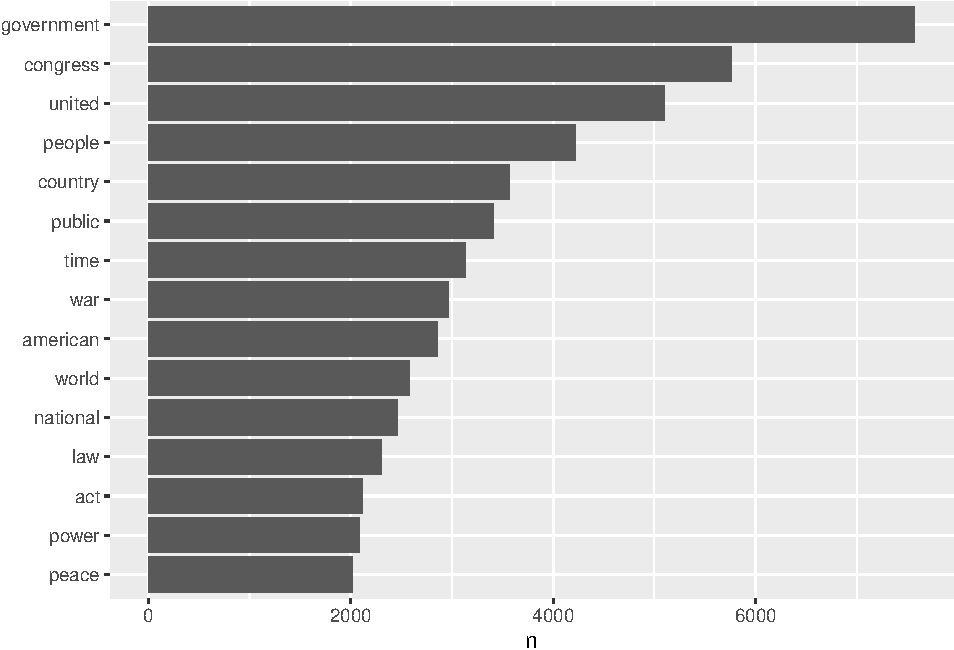
\includegraphics{R-text-analysis_files/figure-latex/unnamed-chunk-5-1.pdf}

What if we're interested in most used words per speech?

\begin{Shaded}
\begin{Highlighting}[]
\CommentTok{# Count words by book}
\NormalTok{doc_words <-}\StringTok{ }\NormalTok{tidy_sotu_words }\OperatorTok
\StringTok{  }\KeywordTok{count}\NormalTok{(doc_id, word, }\DataTypeTok{sort =} \OtherTok{TRUE}\NormalTok{)}

\CommentTok{# Calculate the total number of words by book and save them to a tibble}
\NormalTok{total_words <-}\StringTok{ }\NormalTok{doc_words }\OperatorTok
\StringTok{  }\KeywordTok{group_by}\NormalTok{(doc_id) }\OperatorTok
\StringTok{  }\KeywordTok{summarize}\NormalTok{(}\DataTypeTok{total =} \KeywordTok{sum}\NormalTok{(n))}

\CommentTok{# Join the total column with the rest of the data so we can calculate frequency}
\NormalTok{doc_words <-}\StringTok{ }\KeywordTok{left_join}\NormalTok{(doc_words, total_words)}

\NormalTok{doc_words }
\end{Highlighting}
\end{Shaded}

\begin{verbatim}
#> # A tibble: 352,846 x 4
#>    doc_id                       word               n total
#>    <chr>                        <chr>          <int> <int>
#>  1 harry-s-truman-1946.txt      dollars          207 12614
#>  2 jimmy-carter-1980b.txt       congress         204 16128
#>  3 harry-s-truman-1946.txt      war              201 12614
#>  4 william-howard-taft-1910.txt government       164 11178
#>  5 james-k-polk-1846.txt        mexico           158  7023
#>  6 richard-m-nixon-1974b.txt    federal          141  9996
#>  7 harry-s-truman-1946.txt      million          138 12614
#>  8 harry-s-truman-1946.txt      fiscal           129 12614
#>  9 jimmy-carter-1981.txt        administration   129 16595
#> 10 william-howard-taft-1912.txt government       129 10215
#> # ... with 352,836 more rows
\end{verbatim}

Let's graph the top words per book.

\begin{Shaded}
\begin{Highlighting}[]
\NormalTok{doc_words }\OperatorTok\StringTok{ }
\StringTok{  }\KeywordTok{filter}\NormalTok{(n }\OperatorTok{>}\StringTok{ }\DecValTok{100}\NormalTok{) }\OperatorTok
\StringTok{  }\KeywordTok{ggplot}\NormalTok{(}\KeywordTok{aes}\NormalTok{(word, n, }\DataTypeTok{fill =}\NormalTok{ doc_id)) }\OperatorTok{+}
\StringTok{  }\KeywordTok{geom_col}\NormalTok{() }\OperatorTok{+}\StringTok{ }
\StringTok{  }\KeywordTok{xlab}\NormalTok{(}\OtherTok{NULL}\NormalTok{) }\OperatorTok{+}
\StringTok{  }\KeywordTok{coord_flip}\NormalTok{()}
\end{Highlighting}
\end{Shaded}

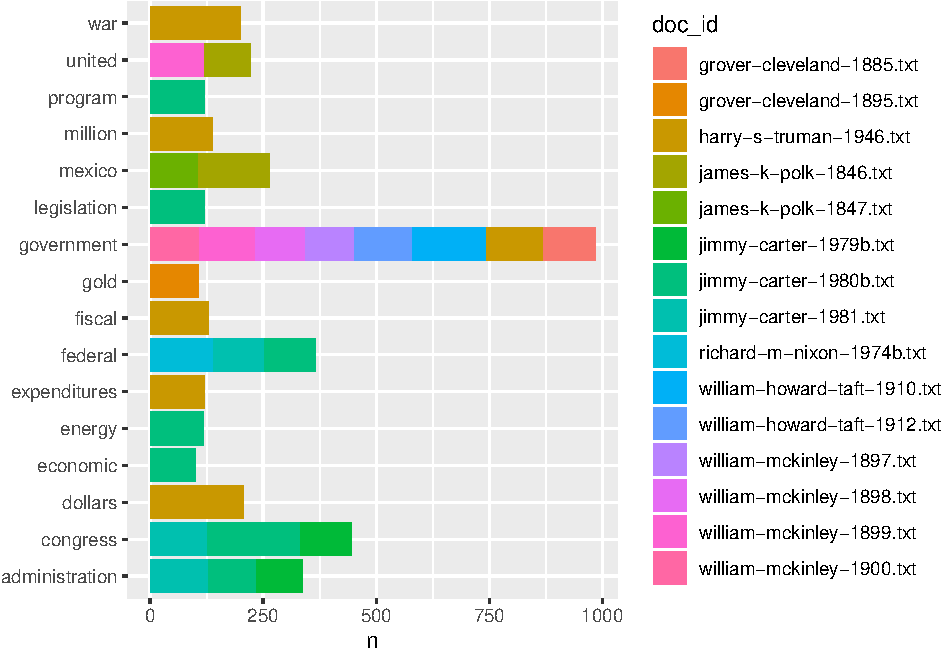
\includegraphics{R-text-analysis_files/figure-latex/unnamed-chunk-7-1.pdf}

That's cool looking, but let's split it into facets so we can see by speech.

\begin{Shaded}
\begin{Highlighting}[]
\NormalTok{doc_words }\OperatorTok\StringTok{ }
\StringTok{  }\KeywordTok{filter}\NormalTok{(n }\OperatorTok{>}\StringTok{ }\DecValTok{100}\NormalTok{) }\OperatorTok
\StringTok{  }\KeywordTok{ggplot}\NormalTok{(}\KeywordTok{aes}\NormalTok{(word, n, }\DataTypeTok{fill =}\NormalTok{ doc_id)) }\OperatorTok{+}
\StringTok{  }\KeywordTok{geom_col}\NormalTok{(}\DataTypeTok{show.legend =} \OtherTok{FALSE}\NormalTok{) }\OperatorTok{+}\StringTok{ }
\StringTok{  }\KeywordTok{xlab}\NormalTok{(}\OtherTok{NULL}\NormalTok{) }\OperatorTok{+}
\StringTok{  }\KeywordTok{facet_wrap}\NormalTok{(}\OperatorTok{~}\NormalTok{doc_id, }\DataTypeTok{ncol =} \DecValTok{2}\NormalTok{) }\OperatorTok{+}\StringTok{ }
\StringTok{  }\KeywordTok{theme}\NormalTok{(}\DataTypeTok{axis.text.x =} \KeywordTok{element_text}\NormalTok{(}\DataTypeTok{angle =} \DecValTok{90}\NormalTok{, }\DataTypeTok{hjust =} \DecValTok{1}\NormalTok{))}
\end{Highlighting}
\end{Shaded}

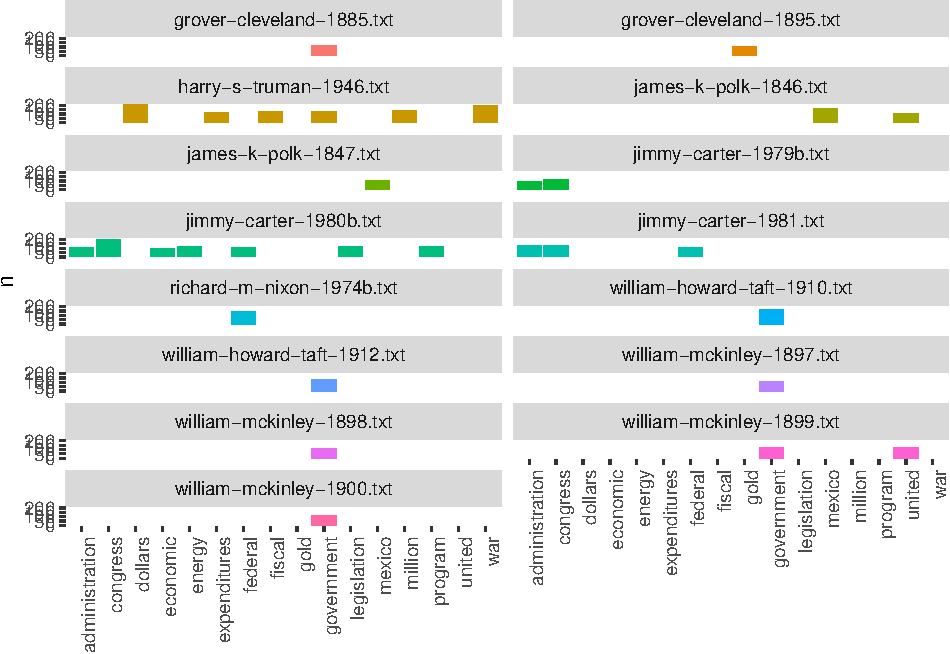
\includegraphics{R-text-analysis_files/figure-latex/unnamed-chunk-8-1.pdf}

We could keep cleaning this figure up by setting some minimum sizing, determining the spacing between y-axis labels better, and so forth, but for now we'll accept it as showing some sense of variation across speeches where certain words are used most.

What if we want to check the most common words per speech for a single president? We could filter this \texttt{doc\_words} dataset based on the president's name being in the doc\_id, but I think it's easier to filter from the initial tidy data and recount.

\begin{Shaded}
\begin{Highlighting}[]
\NormalTok{tidy_sotu_words }\OperatorTok
\StringTok{  }\KeywordTok{filter}\NormalTok{(president }\OperatorTok{==}\StringTok{ "Barack Obama"}\NormalTok{) }\OperatorTok
\StringTok{  }\KeywordTok{count}\NormalTok{(doc_id, word, }\DataTypeTok{sort =} \OtherTok{TRUE}\NormalTok{) }\OperatorTok
\StringTok{  }\KeywordTok{filter}\NormalTok{(n }\OperatorTok{>}\StringTok{ }\DecValTok{20}\NormalTok{) }\OperatorTok
\StringTok{  }\KeywordTok{ggplot}\NormalTok{(}\KeywordTok{aes}\NormalTok{(word, n, }\DataTypeTok{fill=}\NormalTok{doc_id)) }\OperatorTok{+}
\StringTok{  }\KeywordTok{geom_col}\NormalTok{() }\OperatorTok{+}
\StringTok{  }\KeywordTok{facet_wrap}\NormalTok{(}\OperatorTok{~}\NormalTok{doc_id, }\DataTypeTok{ncol =} \DecValTok{2}\NormalTok{) }\OperatorTok{+}\StringTok{ }
\StringTok{  }\KeywordTok{theme}\NormalTok{(}\DataTypeTok{axis.text.x =} \KeywordTok{element_text}\NormalTok{(}\DataTypeTok{angle =} \DecValTok{90}\NormalTok{, }\DataTypeTok{hjust =} \DecValTok{1}\NormalTok{))}
\end{Highlighting}
\end{Shaded}

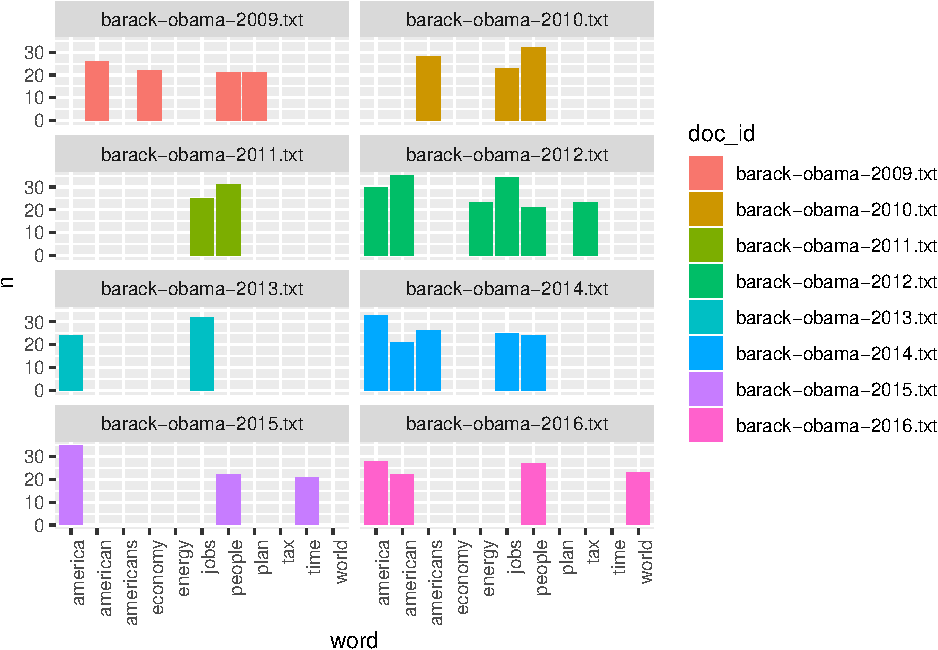
\includegraphics{R-text-analysis_files/figure-latex/unnamed-chunk-9-1.pdf}

\hypertarget{term-frequency}{%
\section{Term frequency}\label{term-frequency}}

Sometimes, a raw count of a word is less important than understanding how often that word appears in respect to the total number of words in a text. This ratio would be the \textbf{term frequency}.

\begin{Shaded}
\begin{Highlighting}[]
\NormalTok{doc_words <-}\StringTok{ }\NormalTok{doc_words }\OperatorTok
\StringTok{  }\KeywordTok{mutate}\NormalTok{(}\DataTypeTok{term_freq =}\NormalTok{ n }\OperatorTok{/}\StringTok{ }\NormalTok{total)}

\NormalTok{doc_words }
\end{Highlighting}
\end{Shaded}

\begin{verbatim}
#> # A tibble: 352,846 x 5
#>    doc_id                       word               n total term_freq
#>    <chr>                        <chr>          <int> <int>     <dbl>
#>  1 harry-s-truman-1946.txt      dollars          207 12614   0.0164 
#>  2 jimmy-carter-1980b.txt       congress         204 16128   0.0126 
#>  3 harry-s-truman-1946.txt      war              201 12614   0.0159 
#>  4 william-howard-taft-1910.txt government       164 11178   0.0147 
#>  5 james-k-polk-1846.txt        mexico           158  7023   0.0225 
#>  6 richard-m-nixon-1974b.txt    federal          141  9996   0.0141 
#>  7 harry-s-truman-1946.txt      million          138 12614   0.0109 
#>  8 harry-s-truman-1946.txt      fiscal           129 12614   0.0102 
#>  9 jimmy-carter-1981.txt        administration   129 16595   0.00777
#> 10 william-howard-taft-1912.txt government       129 10215   0.0126 
#> # ... with 352,836 more rows
\end{verbatim}

Let's graph the term frequency for one of these speeches so we can understand the frequency distribution of words over a text.

\begin{Shaded}
\begin{Highlighting}[]
\NormalTok{doc_words }\OperatorTok
\StringTok{  }\KeywordTok{filter}\NormalTok{(doc_id }\OperatorTok{==}\StringTok{ "harry-s-truman-1946.txt"}\NormalTok{) }\OperatorTok
\StringTok{  }\KeywordTok{ggplot}\NormalTok{(}\KeywordTok{aes}\NormalTok{(term_freq)) }\OperatorTok{+}
\StringTok{  }\KeywordTok{geom_histogram}\NormalTok{(}\DataTypeTok{show.legend =} \OtherTok{FALSE}\NormalTok{) }\OperatorTok{+}
\StringTok{  }\KeywordTok{xlim}\NormalTok{(}\OtherTok{NA}\NormalTok{, }\FloatTok{.012}\NormalTok{)}
\end{Highlighting}
\end{Shaded}

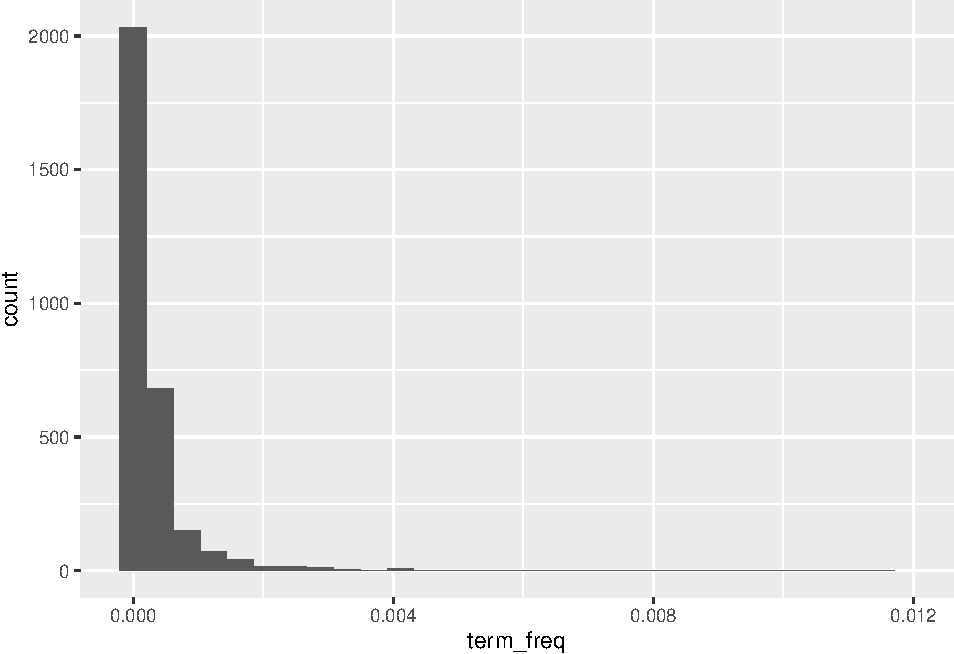
\includegraphics{R-text-analysis_files/figure-latex/unnamed-chunk-11-1.pdf}

This distribution makes sense. Most words are used relatively rarely in a text. Only a few have a high term frequency.

We could keep filtering this data to see which terms have high frequency, thus maybe increased significance, for different presidents and different particular speeches. We could also subset based on decade, and get a sense of what was important in each decade. We're going to take a slightly different approach though. We've been looking at term frequency per document. What if we want to know about words that seem more important based on the contents of the entire corpus?

\hypertarget{tf-idf}{%
\section{Tf-idf}\label{tf-idf}}

For this, we can use term-frequency according to inverse document frequency (tf-idf). Tf-idf measures how important a word is within a corpus by scaling term frequency per document according to the inverse of the term's document frequency (number of documents within the corpus in which the term appears divided by the number of documents).

We could write our own function for tf-idf, but in this case we'll take advantage of tidytext's implementation.

\begin{Shaded}
\begin{Highlighting}[]
\NormalTok{doc_words <-}\StringTok{ }\NormalTok{doc_words }\OperatorTok
\StringTok{  }\KeywordTok{bind_tf_idf}\NormalTok{(word, doc_id, n)}

\NormalTok{doc_words}
\end{Highlighting}
\end{Shaded}

\begin{verbatim}
#> # A tibble: 352,846 x 8
#>    doc_id           word          n total term_freq      tf     idf  tf_idf
#>    <chr>            <chr>     <int> <int>     <dbl>   <dbl>   <dbl>   <dbl>
#>  1 harry-s-truman-~ dollars     207 12614   0.0164  0.0164  0.612   1.00e-2
#>  2 jimmy-carter-19~ congress    204 16128   0.0126  0.0126  0.00425 5.37e-5
#>  3 harry-s-truman-~ war         201 12614   0.0159  0.0159  0.0345  5.50e-4
#>  4 william-howard-~ governme~   164 11178   0.0147  0.0147  0.00425 6.23e-5
#>  5 james-k-polk-18~ mexico      158  7023   0.0225  0.0225  0.810   1.82e-2
#>  6 richard-m-nixon~ federal     141  9996   0.0141  0.0141  0.293   4.14e-3
#>  7 harry-s-truman-~ million     138 12614   0.0109  0.0109  0.728   7.96e-3
#>  8 harry-s-truman-~ fiscal      129 12614   0.0102  0.0102  0.494   5.05e-3
#>  9 jimmy-carter-19~ administ~   129 16595   0.00777 0.00777 0.282   2.19e-3
#> 10 william-howard-~ governme~   129 10215   0.0126  0.0126  0.00425 5.36e-5
#> # ... with 352,836 more rows
\end{verbatim}

The tf-idf value will be:

\begin{itemize}
\tightlist
\item
  lower for words that appear in many documents in the corpus, and lowest when the word occurs in virtually all documents.
\item
  high for words that appear many times in few documents in the corpus, this lending high discriminatory power to those documents.
\end{itemize}

Let's look at some of the words in the corpus that have the highest tf-idf scores, which means words that are particularly distinctive for their documents.

\begin{Shaded}
\begin{Highlighting}[]
\NormalTok{doc_words }\OperatorTok
\StringTok{  }\KeywordTok{select}\NormalTok{(}\OperatorTok{-}\NormalTok{total) }\OperatorTok
\StringTok{  }\KeywordTok{arrange}\NormalTok{(}\KeywordTok{desc}\NormalTok{(tf_idf))}
\end{Highlighting}
\end{Shaded}

\begin{verbatim}
#> # A tibble: 352,846 x 7
#>    doc_id                     word         n term_freq      tf   idf tf_idf
#>    <chr>                      <chr>    <int>     <dbl>   <dbl> <dbl>  <dbl>
#>  1 lyndon-b-johnson-1966.txt  vietnam     32   0.0152  0.0152   2.42 0.0367
#>  2 jimmy-carter-1980a.txt     soviet      31   0.0218  0.0218   1.47 0.0321
#>  3 george-w-bush-2003.txt     hussein     19   0.00811 0.00811  3.85 0.0313
#>  4 george-w-bush-2003.txt     saddam      19   0.00811 0.00811  3.67 0.0298
#>  5 franklin-d-roosevelt-1943~ 1942        13   0.00758 0.00758  3.85 0.0292
#>  6 dwight-d-eisenhower-1961.~ 1953        23   0.00747 0.00747  3.85 0.0288
#>  7 john-adams-1800.txt        gentlem~     8   0.0153  0.0153   1.80 0.0275
#>  8 benjamin-harrison-1892.txt 1892        40   0.00741 0.00741  3.52 0.0261
#>  9 franklin-d-roosevelt-1942~ hitler       7   0.00527 0.00527  4.77 0.0251
#> 10 herbert-hoover-1930.txt    1928        14   0.00711 0.00711  3.52 0.0250
#> # ... with 352,836 more rows
\end{verbatim}

These results seem appropriate given our history. To understand the occurrence of the years we might need to look more closely at the speeches themselves, and determine whether the years are significant or whether they need to be removed from the text. It might be that even if they don't need to be removed from the text overall, they still need to be filtered out within the context of this analysis.

In the same way that we narrowed our analysis to Obama speeches earlier, we could subset the corpus before we calculate the tf-idf score to understand which words are most important for a single president within their sotu speeches. Let's do that for Obama.

\begin{Shaded}
\begin{Highlighting}[]
\NormalTok{obama_tf_idf <-}\StringTok{ }\NormalTok{tidy_sotu_words }\OperatorTok
\StringTok{  }\KeywordTok{filter}\NormalTok{(president }\OperatorTok{==}\StringTok{ "Barack Obama"}\NormalTok{) }\OperatorTok
\StringTok{  }\KeywordTok{count}\NormalTok{(doc_id, word, }\DataTypeTok{sort =} \OtherTok{TRUE}\NormalTok{) }\OperatorTok
\StringTok{  }\KeywordTok{bind_tf_idf}\NormalTok{(word, doc_id, n) }\OperatorTok
\StringTok{  }\KeywordTok{arrange}\NormalTok{(}\KeywordTok{desc}\NormalTok{(tf_idf))}

\NormalTok{obama_tf_idf}
\end{Highlighting}
\end{Shaded}

\begin{verbatim}
#> # A tibble: 10,656 x 6
#>    doc_id                word          n      tf   idf  tf_idf
#>    <chr>                 <chr>     <int>   <dbl> <dbl>   <dbl>
#>  1 barack-obama-2016.txt voices        8 0.00372  2.08 0.00773
#>  2 barack-obama-2014.txt cory          9 0.00322  2.08 0.00671
#>  3 barack-obama-2015.txt rebekah       7 0.00273  2.08 0.00567
#>  4 barack-obama-2012.txt unit          7 0.00255  2.08 0.00531
#>  5 barack-obama-2016.txt isil          8 0.00372  1.39 0.00515
#>  6 barack-obama-2009.txt restart       5 0.00221  2.08 0.00460
#>  7 barack-obama-2013.txt reduction     6 0.00220  2.08 0.00458
#>  8 barack-obama-2015.txt childcare     8 0.00312  1.39 0.00432
#>  9 barack-obama-2011.txt brandon       5 0.00197  2.08 0.00409
#> 10 barack-obama-2015.txt economics     5 0.00195  2.08 0.00405
#> # ... with 10,646 more rows
\end{verbatim}

Based on what you know of the Obama years and sotu speeches generally, how would you interpret these results?

Let's try graphing these results, showing the top tf-idf terms per speech for Obama's speeches.

\begin{Shaded}
\begin{Highlighting}[]
\NormalTok{obama_tf_idf }\OperatorTok
\StringTok{  }\KeywordTok{group_by}\NormalTok{(doc_id) }\OperatorTok
\StringTok{  }\KeywordTok{mutate}\NormalTok{(}\DataTypeTok{word =} \KeywordTok{factor}\NormalTok{(word, }\DataTypeTok{levels =} \KeywordTok{rev}\NormalTok{(}\KeywordTok{unique}\NormalTok{(word)))) }\OperatorTok\StringTok{ }
\StringTok{  }\KeywordTok{group_by}\NormalTok{(doc_id) }\OperatorTok\StringTok{ }
\StringTok{  }\KeywordTok{top_n}\NormalTok{(}\DecValTok{5}\NormalTok{) }\OperatorTok\StringTok{ }
\StringTok{  }\KeywordTok{ungroup}\NormalTok{() }\OperatorTok
\StringTok{  }\KeywordTok{ggplot}\NormalTok{(}\KeywordTok{aes}\NormalTok{(word, tf_idf, }\DataTypeTok{fill =}\NormalTok{ doc_id)) }\OperatorTok{+}
\StringTok{  }\KeywordTok{geom_col}\NormalTok{(}\DataTypeTok{show.legend =} \OtherTok{FALSE}\NormalTok{) }\OperatorTok{+}
\StringTok{  }\KeywordTok{labs}\NormalTok{(}\DataTypeTok{x =} \OtherTok{NULL}\NormalTok{, }\DataTypeTok{y =} \StringTok{"tf-idf"}\NormalTok{) }\OperatorTok{+}
\StringTok{  }\KeywordTok{facet_wrap}\NormalTok{(}\OperatorTok{~}\NormalTok{doc_id, }\DataTypeTok{ncol =} \DecValTok{2}\NormalTok{, }\DataTypeTok{scales =} \StringTok{"free"}\NormalTok{) }\OperatorTok{+}
\StringTok{  }\KeywordTok{coord_flip}\NormalTok{() }\OperatorTok{+}\StringTok{ }
\StringTok{  }\KeywordTok{theme}\NormalTok{(}\DataTypeTok{axis.text.y =} \KeywordTok{element_text}\NormalTok{(}\DataTypeTok{angle =} \DecValTok{45}\NormalTok{)) }
\end{Highlighting}
\end{Shaded}

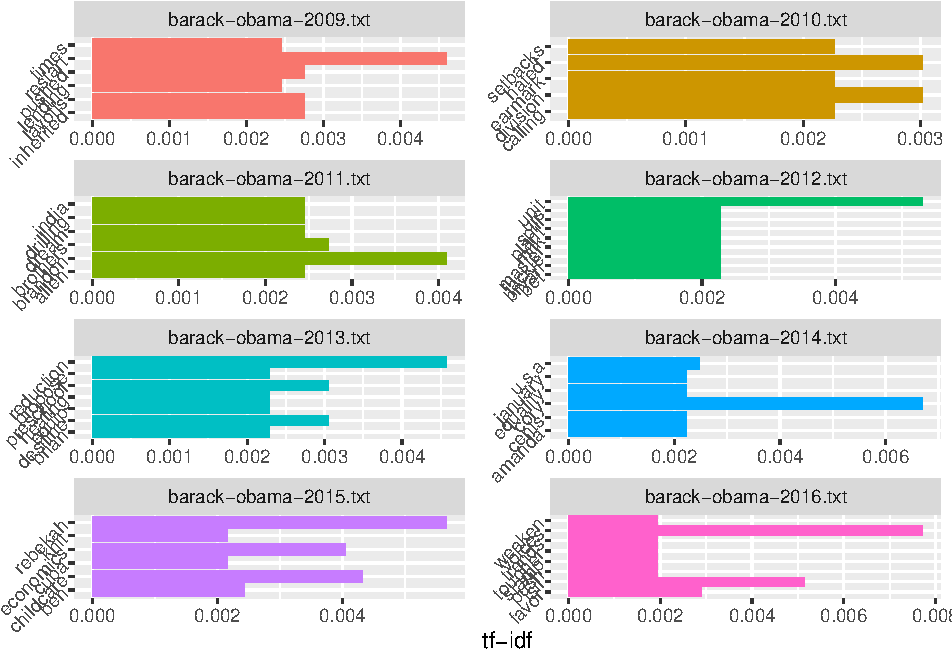
\includegraphics{R-text-analysis_files/figure-latex/unnamed-chunk-15-1.pdf}

\hypertarget{n-grams}{%
\section{N-Grams}\label{n-grams}}

We mentioned n-grams in the intro, but let's revisit them here and take a look at the most common bigrams in the speeches. Remember this is what we get back:

\begin{Shaded}
\begin{Highlighting}[]
\NormalTok{sotu_whole }\OperatorTok
\StringTok{  }\KeywordTok{unnest_tokens}\NormalTok{(bigram, text, }\DataTypeTok{token =} \StringTok{"ngrams"}\NormalTok{, }\DataTypeTok{n =} \DecValTok{2}\NormalTok{) }\CommentTok{# create bigram}
\end{Highlighting}
\end{Shaded}

\begin{verbatim}
#> # A tibble: 1,964,976 x 7
#>    president     year years_active party  sotu_type doc_id       bigram    
#>    <chr>        <int> <chr>        <chr>  <chr>     <chr>        <chr>     
#>  1 Abraham Lin~  1861 1861-1865    Repub~ written   abraham-lin~ fellow ci~
#>  2 Abraham Lin~  1861 1861-1865    Repub~ written   abraham-lin~ citizens ~
#>  3 Abraham Lin~  1861 1861-1865    Repub~ written   abraham-lin~ of the    
#>  4 Abraham Lin~  1861 1861-1865    Repub~ written   abraham-lin~ the senate
#>  5 Abraham Lin~  1861 1861-1865    Repub~ written   abraham-lin~ senate and
#>  6 Abraham Lin~  1861 1861-1865    Repub~ written   abraham-lin~ and house 
#>  7 Abraham Lin~  1861 1861-1865    Repub~ written   abraham-lin~ house of  
#>  8 Abraham Lin~  1861 1861-1865    Repub~ written   abraham-lin~ of repres~
#>  9 Abraham Lin~  1861 1861-1865    Repub~ written   abraham-lin~ represent~
#> 10 Abraham Lin~  1861 1861-1865    Repub~ written   abraham-lin~ in the    
#> # ... with 1,964,966 more rows
\end{verbatim}

Let's see the most common bigrams:

\begin{Shaded}
\begin{Highlighting}[]
\NormalTok{sotu_whole }\OperatorTok
\StringTok{  }\KeywordTok{unnest_tokens}\NormalTok{(bigram, text, }\DataTypeTok{token =} \StringTok{"ngrams"}\NormalTok{, }\DataTypeTok{n =} \DecValTok{2}\NormalTok{) }\OperatorTok\StringTok{ }
\StringTok{  }\KeywordTok{count}\NormalTok{(bigram, }\DataTypeTok{sort =} \OtherTok{TRUE}\NormalTok{) }\CommentTok{# count ocurrences and sord descending}
\end{Highlighting}
\end{Shaded}

\begin{verbatim}
#> # A tibble: 469,092 x 2
#>    bigram            n
#>    <chr>         <int>
#>  1 of the        33610
#>  2 in the        12499
#>  3 to the        11643
#>  4 for the        6892
#>  5 and the        6224
#>  6 by the         5606
#>  7 of our         5172
#>  8 the united     4767
#>  9 united states  4760
#> 10 it is          4756
#> # ... with 469,082 more rows
\end{verbatim}

Ok, so we again need to remove the stopwords. This time let's use dplyr's \texttt{filter} function for this. And before that we will \texttt{separate} the two words into two columns.

\begin{Shaded}
\begin{Highlighting}[]
\NormalTok{sotu_bigrams <-}\StringTok{ }\NormalTok{sotu_whole }\OperatorTok
\StringTok{  }\KeywordTok{unnest_tokens}\NormalTok{(bigram, text, }\DataTypeTok{token =} \StringTok{"ngrams"}\NormalTok{, }\DataTypeTok{n =} \DecValTok{2}\NormalTok{) }\OperatorTok\StringTok{ }
\StringTok{  }\KeywordTok{separate}\NormalTok{(bigram, }\KeywordTok{c}\NormalTok{(}\StringTok{"word1"}\NormalTok{, }\StringTok{"word2"}\NormalTok{), }\DataTypeTok{sep =} \StringTok{" "}\NormalTok{) }\OperatorTok\StringTok{ }\CommentTok{# separate into cols}
\StringTok{  }\KeywordTok{filter}\NormalTok{(}\OperatorTok{!}\NormalTok{word1 }\OperatorTok\StringTok{ }\NormalTok{stop_words}\OperatorTok{$}\NormalTok{word) }\OperatorTok\StringTok{ }\CommentTok{# remove stopwords}
\StringTok{  }\KeywordTok{filter}\NormalTok{(}\OperatorTok{!}\NormalTok{word2 }\OperatorTok\StringTok{ }\NormalTok{stop_words}\OperatorTok{$}\NormalTok{word)}

\NormalTok{sotu_bigrams }\OperatorTok\StringTok{ }
\StringTok{  }\KeywordTok{count}\NormalTok{(word1, word2, }\DataTypeTok{sort =} \OtherTok{TRUE}\NormalTok{)}
\end{Highlighting}
\end{Shaded}

\begin{verbatim}
#> # A tibble: 129,622 x 3
#>    word1    word2          n
#>    <chr>    <chr>      <int>
#>  1 federal  government   479
#>  2 american people       428
#>  3 june     30           325
#>  4 fellow   citizens     296
#>  5 public   debt         283
#>  6 public   lands        256
#>  7 health   care         240
#>  8 social   security     232
#>  9 post     office       202
#> 10 annual   message      200
#> # ... with 129,612 more rows
\end{verbatim}

(Bonus question: What happened on that June 30th?)

A bigram can also be treated as a term in a document in the same way that we treated individual words. That means we can look at tf-idf values in the same way.

First we will re-unite the two word columns again, and then generate the tf-idf count as above.

\begin{Shaded}
\begin{Highlighting}[]
\NormalTok{bigram_tf_idf <-}\StringTok{ }\NormalTok{sotu_bigrams }\OperatorTok
\StringTok{  }\KeywordTok{unite}\NormalTok{(bigram, word1, word2, }\DataTypeTok{sep =} \StringTok{" "}\NormalTok{) }\OperatorTok\StringTok{ }\CommentTok{# combine columns}
\StringTok{  }\KeywordTok{count}\NormalTok{(president, bigram) }\OperatorTok
\StringTok{  }\KeywordTok{bind_tf_idf}\NormalTok{(bigram, president, n) }\OperatorTok
\StringTok{  }\KeywordTok{arrange}\NormalTok{(}\KeywordTok{desc}\NormalTok{(tf_idf))}
\end{Highlighting}
\end{Shaded}

What makes the speeches of different presidents unique?

Let's pick a few presidents and plot their highest scoring tf-idf values here.

\begin{Shaded}
\begin{Highlighting}[]
\NormalTok{potus <-}\StringTok{ }\KeywordTok{c}\NormalTok{(}\StringTok{"John F. Kennedy"}\NormalTok{, }\StringTok{"Richard M. Nixon"}\NormalTok{, }\StringTok{"George Bush"}\NormalTok{, }\StringTok{"George W. Bush"}\NormalTok{)}

\NormalTok{bigram_tf_idf }\OperatorTok
\StringTok{  }\KeywordTok{filter}\NormalTok{(president }\OperatorTok\StringTok{ }\NormalTok{potus) }\OperatorTok\StringTok{ }
\StringTok{  }\KeywordTok{group_by}\NormalTok{(president) }\OperatorTok\StringTok{ }
\StringTok{  }\KeywordTok{top_n}\NormalTok{(}\DecValTok{20}\NormalTok{) }\OperatorTok\StringTok{ }
\StringTok{  }\KeywordTok{ggplot}\NormalTok{(}\KeywordTok{aes}\NormalTok{(}\KeywordTok{reorder}\NormalTok{(bigram, tf_idf), tf_idf, }\DataTypeTok{fill =}\NormalTok{ president)) }\OperatorTok{+}
\StringTok{  }\KeywordTok{geom_col}\NormalTok{(}\DataTypeTok{show.legend =} \OtherTok{FALSE}\NormalTok{) }\OperatorTok{+}
\StringTok{  }\KeywordTok{labs}\NormalTok{(}\DataTypeTok{x =} \OtherTok{NULL}\NormalTok{, }\DataTypeTok{y =} \StringTok{"tf-idf"}\NormalTok{) }\OperatorTok{+}
\StringTok{  }\KeywordTok{facet_wrap}\NormalTok{(}\OperatorTok{~}\NormalTok{president, }\DataTypeTok{scales =} \StringTok{"free"}\NormalTok{, }\DataTypeTok{nrow =} \DecValTok{2}\NormalTok{) }\OperatorTok{+}
\StringTok{  }\KeywordTok{coord_flip}\NormalTok{()}
\end{Highlighting}
\end{Shaded}

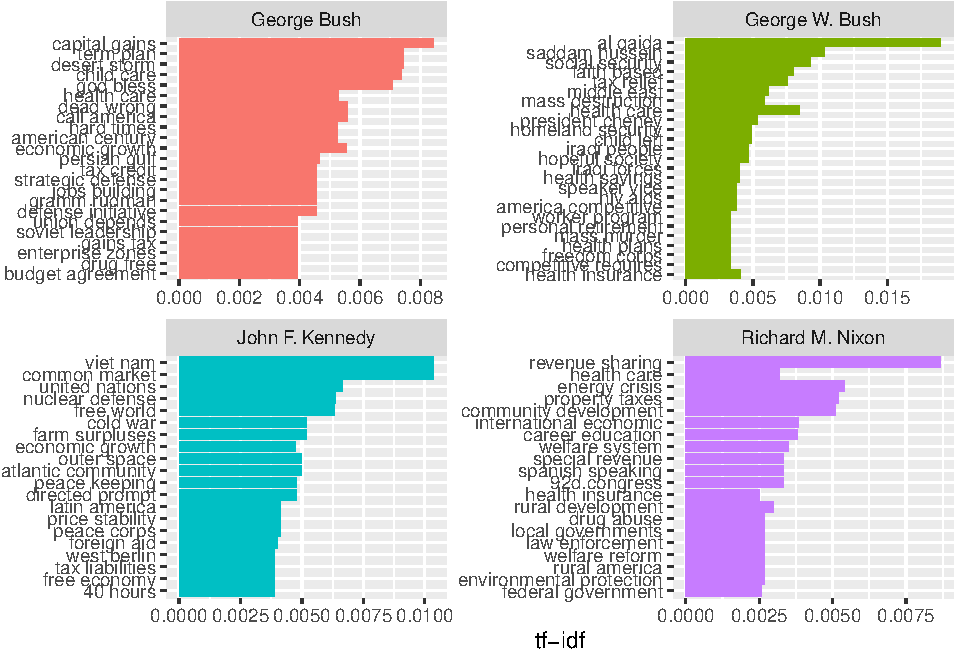
\includegraphics{R-text-analysis_files/figure-latex/bigram-tf-idf-plot-1.pdf}

\hypertarget{co-occurrence}{%
\section{Co-occurrence}\label{co-occurrence}}

Co-occurrences give us a sense of words that appear in the same text, but not necessarily next to each other.

For this section we will make use of the \texttt{widyr} package. It allows us to turn our table into a wide matrix. In our case that matrix will be made up of the individual words and the cell values will be the counts of how many times they co-occur. Then we will turn the matrix back into a tidy form, where each row contains the word pairs and the count of their co-occurrence. This lets us count common pairs of words co-appearing within the same speech.

The function which helps us do this is the \texttt{pairwise\_count()} function.

Since processing the entire corpus would take too long here, we will only look at the last 20 words of each speech.

\begin{Shaded}
\begin{Highlighting}[]
\KeywordTok{library}\NormalTok{(widyr)}

\CommentTok{# extract last 100 words from text}
\NormalTok{sotu_whole}\OperatorTok{$}\NormalTok{speech_end <-}\StringTok{ }\KeywordTok{word}\NormalTok{(sotu_whole}\OperatorTok{$}\NormalTok{text, }\DecValTok{-100}\NormalTok{, }\DataTypeTok{end =} \DecValTok{-1}\NormalTok{)}

\NormalTok{sotu_word_pairs <-}\StringTok{ }\NormalTok{sotu_whole }\OperatorTok\StringTok{ }
\StringTok{  }\KeywordTok{unnest_tokens}\NormalTok{(word, speech_end) }\OperatorTok\StringTok{ }
\StringTok{  }\KeywordTok{filter}\NormalTok{(}\OperatorTok{!}\NormalTok{word }\OperatorTok\StringTok{ }\NormalTok{stop_words}\OperatorTok{$}\NormalTok{word) }\OperatorTok\StringTok{ }\CommentTok{# remove stopwords}
\StringTok{  }\KeywordTok{pairwise_count}\NormalTok{(word, doc_id, }\DataTypeTok{sort =} \OtherTok{TRUE}\NormalTok{, }\DataTypeTok{upper =} \OtherTok{FALSE}\NormalTok{) }\CommentTok{# don't include upper triangle of matrix}

\NormalTok{sotu_word_pairs}
\end{Highlighting}
\end{Shaded}

\begin{verbatim}
#> # A tibble: 125,576 x 3
#>    item1      item2       n
#>    <chr>      <chr>   <dbl>
#>  1 god        bless      37
#>  2 god        america    35
#>  3 bless      america    30
#>  4 people     country    26
#>  5 world      god        22
#>  6 god        people     22
#>  7 government people     21
#>  8 congress   people     21
#>  9 public     country    21
#> 10 god        nation     21
#> # ... with 125,566 more rows
\end{verbatim}

To plot the co-occurrence network, we use the \texttt{igraph} library to convert our table into a network graph and \texttt{ggraph} which adds functionality to ggplot and makes it easier to create a network plot.

\begin{Shaded}
\begin{Highlighting}[]
\KeywordTok{library}\NormalTok{(igraph)}
\KeywordTok{library}\NormalTok{(ggraph)}

\NormalTok{sotu_word_pairs }\OperatorTok\StringTok{ }
\StringTok{  }\KeywordTok{filter}\NormalTok{(n }\OperatorTok{>=}\StringTok{ }\DecValTok{10}\NormalTok{) }\OperatorTok\StringTok{  }\CommentTok{# only word pairs that occur 10 or more times}
\StringTok{  }\KeywordTok{graph_from_data_frame}\NormalTok{() }\OperatorTok\StringTok{ }\CommentTok{#convert to graph}
\StringTok{  }\KeywordTok{ggraph}\NormalTok{(}\DataTypeTok{layout =} \StringTok{"fr"}\NormalTok{) }\OperatorTok{+}\StringTok{ }\CommentTok{# place nodes according to the force-directed algorithm of Fruchterman and Reingold}
\StringTok{  }\KeywordTok{geom_edge_link}\NormalTok{(}\KeywordTok{aes}\NormalTok{(}\DataTypeTok{edge_alpha =}\NormalTok{ n, }\DataTypeTok{edge_width =}\NormalTok{ n), }\DataTypeTok{edge_colour =} \StringTok{"tomato"}\NormalTok{) }\OperatorTok{+}
\StringTok{  }\KeywordTok{geom_node_point}\NormalTok{(}\DataTypeTok{size =} \DecValTok{5}\NormalTok{) }\OperatorTok{+}
\StringTok{  }\KeywordTok{geom_node_text}\NormalTok{(}\KeywordTok{aes}\NormalTok{(}\DataTypeTok{label =}\NormalTok{ name), }\DataTypeTok{repel =} \OtherTok{TRUE}\NormalTok{, }
                 \DataTypeTok{point.padding =} \KeywordTok{unit}\NormalTok{(}\FloatTok{0.2}\NormalTok{, }\StringTok{"lines"}\NormalTok{)) }\OperatorTok{+}
\StringTok{  }\KeywordTok{theme_void}\NormalTok{()}
\end{Highlighting}
\end{Shaded}

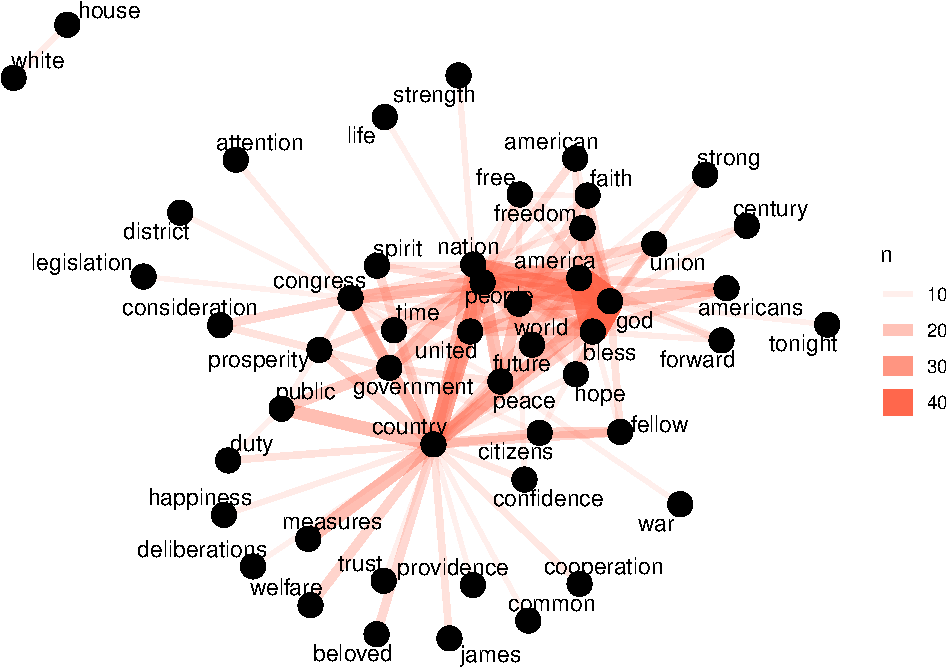
\includegraphics{R-text-analysis_files/figure-latex/plot-network-1.pdf}

There are alternative approaches for this as well. See for example the \texttt{findAssocs} function in the \texttt{tm} package.

\hypertarget{document-term-matrix}{%
\section{Document-Term Matrix}\label{document-term-matrix}}

A \href{https://en.wikipedia.org/wiki/Document-term_matrix}{document-term matrix (DTM)} is a format which is frequently used in text analysis. It is a matrix where we can see the counts of each term per document. In a DTM each row represents a document, each column represents a term, and the cell values are the counts of the occurrences of the term for the particular document.

\texttt{tidytext} provides functionality to convert to and from DTMs, if for example, your analyis requires specific functions that require you to use a different R package which only works with DTM objects.

The \texttt{cast\_dtm} function can be used to create a DTM object from a tidy table.

Let's assume that for some reason we want to use the \texttt{findAssoc} function from the \texttt{tm} package.

First we use dplyr to create a table with the document name, the term, and the count.

\begin{Shaded}
\begin{Highlighting}[]
\CommentTok{# make a table with document, term, count}
\NormalTok{tidy_sotu_words }\OperatorTok\StringTok{ }
\StringTok{  }\KeywordTok{count}\NormalTok{(doc_id, word) }
\end{Highlighting}
\end{Shaded}

\begin{verbatim}
#> # A tibble: 352,846 x 3
#>    doc_id                   word               n
#>    <chr>                    <chr>          <int>
#>  1 abraham-lincoln-1861.txt 1,470,018          1
#>  2 abraham-lincoln-1861.txt 1,500              1
#>  3 abraham-lincoln-1861.txt 100,000            1
#>  4 abraham-lincoln-1861.txt 102,532,509.27     1
#>  5 abraham-lincoln-1861.txt 12,528,000         1
#>  6 abraham-lincoln-1861.txt 13,606,759.11      1
#>  7 abraham-lincoln-1861.txt 1830               1
#>  8 abraham-lincoln-1861.txt 1859               1
#>  9 abraham-lincoln-1861.txt 1860               2
#> 10 abraham-lincoln-1861.txt 1861               6
#> # ... with 352,836 more rows
\end{verbatim}

Now we cast it as a DTM.

\begin{Shaded}
\begin{Highlighting}[]
\NormalTok{sotu_dtm <-}\StringTok{ }\NormalTok{tidy_sotu_words }\OperatorTok\StringTok{ }
\StringTok{  }\KeywordTok{count}\NormalTok{(doc_id, word) }\OperatorTok\StringTok{ }
\StringTok{  }\KeywordTok{cast_dtm}\NormalTok{(doc_id, word, n) }

\KeywordTok{class}\NormalTok{(sotu_dtm)}
\end{Highlighting}
\end{Shaded}

\begin{verbatim}
#> [1] "DocumentTermMatrix"    "simple_triplet_matrix"
\end{verbatim}

Finally, let's use it in the \texttt{tm} package.

\begin{Shaded}
\begin{Highlighting}[]
\KeywordTok{library}\NormalTok{(tm)}

\CommentTok{# look at the terms with tm function}
\KeywordTok{Terms}\NormalTok{(sotu_dtm) }\OperatorTok\StringTok{ }\KeywordTok{tail}\NormalTok{()}
\end{Highlighting}
\end{Shaded}

\begin{verbatim}
#> [1] "queretaro"    "refreshments" "schleswig"    "sedulous"    
#> [5] "subagents"    "transcript"
\end{verbatim}

\begin{Shaded}
\begin{Highlighting}[]
\CommentTok{# most frequent terms}
\KeywordTok{findFreqTerms}\NormalTok{(sotu_dtm, }\DataTypeTok{lowfreq =} \DecValTok{5000}\NormalTok{)}
\end{Highlighting}
\end{Shaded}

\begin{verbatim}
#> [1] "congress"   "government" "united"
\end{verbatim}

\begin{Shaded}
\begin{Highlighting}[]
\CommentTok{# find terms associated with ...}
\KeywordTok{findAssocs}\NormalTok{(sotu_dtm, }\StringTok{"citizen"}\NormalTok{, }\DataTypeTok{corlimit =} \FloatTok{0.5}\NormalTok{)}
\end{Highlighting}
\end{Shaded}

\begin{verbatim}
#> $citizen
#>        laws citizenship  protection   contained    entitled  government 
#>        0.62        0.59        0.56        0.55        0.53        0.53 
#>    citizens  postmaster     careful    question      report       suits 
#>        0.52        0.52        0.51        0.51        0.51        0.51
\end{verbatim}

Conversely, \texttt{tidytext} implements the \texttt{tidy} function (originally from the \texttt{broom} package) to import DocumentTermMatrix objects. Note that it only takes the cells from the DTM that are not 0, so there will be no rows with 0 counts.

\hypertarget{sentiment-analysis}{%
\section{Sentiment analysis}\label{sentiment-analysis}}

\texttt{tidytext} comes with a dataset \texttt{sentiments} which contains several sentiment lexicons, where each word is attributed a certain sentiment, like this:

\begin{Shaded}
\begin{Highlighting}[]
\NormalTok{sentiments}
\end{Highlighting}
\end{Shaded}

\begin{verbatim}
#> # A tibble: 6,786 x 2
#>    word        sentiment
#>    <chr>       <chr>    
#>  1 2-faces     negative 
#>  2 abnormal    negative 
#>  3 abolish     negative 
#>  4 abominable  negative 
#>  5 abominably  negative 
#>  6 abominate   negative 
#>  7 abomination negative 
#>  8 abort       negative 
#>  9 aborted     negative 
#> 10 aborts      negative 
#> # ... with 6,776 more rows
\end{verbatim}

Here we will take a look at how the sentiment of the speeches change over time. We will use the lexicon from \href{https://www.cs.uic.edu/~liub/FBS/sentiment-analysis.html}{Bing Liu and collaborators}, which assigns positive/negative labels for each word:

\begin{Shaded}
\begin{Highlighting}[]
\NormalTok{bing_lex <-}\StringTok{ }\KeywordTok{get_sentiments}\NormalTok{(}\StringTok{"bing"}\NormalTok{)}
\NormalTok{bing_lex}
\end{Highlighting}
\end{Shaded}

\begin{verbatim}
#> # A tibble: 6,786 x 2
#>    word        sentiment
#>    <chr>       <chr>    
#>  1 2-faces     negative 
#>  2 abnormal    negative 
#>  3 abolish     negative 
#>  4 abominable  negative 
#>  5 abominably  negative 
#>  6 abominate   negative 
#>  7 abomination negative 
#>  8 abort       negative 
#>  9 aborted     negative 
#> 10 aborts      negative 
#> # ... with 6,776 more rows
\end{verbatim}

Since this is a regular tibble, we can use these sentiments and join them to the words of our speeches. We will use \texttt{inner\_join} from \texttt{dplyr}. Since our columns to join on have the same name (\texttt{word}) we don't need to explicitly name it.

\begin{Shaded}
\begin{Highlighting}[]
\NormalTok{tidy_sotu_words }\OperatorTok\StringTok{ }
\StringTok{  }\KeywordTok{inner_join}\NormalTok{(bing_lex) }\OperatorTok\StringTok{ }\CommentTok{# join}
\StringTok{  }\KeywordTok{count}\NormalTok{(year, sentiment) }\CommentTok{# group by year and sentiment}
\end{Highlighting}
\end{Shaded}

\begin{verbatim}
#> # A tibble: 450 x 3
#>     year sentiment     n
#>    <int> <chr>     <int>
#>  1  1790 negative     39
#>  2  1790 positive    125
#>  3  1791 negative     52
#>  4  1791 positive    103
#>  5  1792 negative     57
#>  6  1792 positive     78
#>  7  1793 negative     58
#>  8  1793 positive     72
#>  9  1794 negative    110
#> 10  1794 positive    106
#> # ... with 440 more rows
\end{verbatim}

Finally we can visualize it like this:

\begin{Shaded}
\begin{Highlighting}[]
\NormalTok{tidy_sotu_words }\OperatorTok\StringTok{ }
\StringTok{  }\KeywordTok{inner_join}\NormalTok{(bing_lex) }\OperatorTok\StringTok{ }\CommentTok{# join}
\StringTok{  }\KeywordTok{count}\NormalTok{(year, sentiment) }\OperatorTok\StringTok{ }\CommentTok{# group by year and sentiment}
\StringTok{  }\KeywordTok{ggplot}\NormalTok{(}\KeywordTok{aes}\NormalTok{(year, n, }\DataTypeTok{color =}\NormalTok{ sentiment)) }\OperatorTok{+}
\StringTok{    }\KeywordTok{geom_line}\NormalTok{() }\OperatorTok{+}
\StringTok{    }\KeywordTok{scale_x_continuous}\NormalTok{(}\DataTypeTok{breaks =} \KeywordTok{seq}\NormalTok{(}\DecValTok{1790}\NormalTok{, }\DecValTok{2016}\NormalTok{, }\DataTypeTok{by =} \DecValTok{10}\NormalTok{)) }\OperatorTok{+}
\StringTok{    }\KeywordTok{theme}\NormalTok{(}\DataTypeTok{axis.text.x =} \KeywordTok{element_text}\NormalTok{(}\DataTypeTok{angle =} \DecValTok{45}\NormalTok{, }\DataTypeTok{hjust =} \DecValTok{1}\NormalTok{))}
\end{Highlighting}
\end{Shaded}

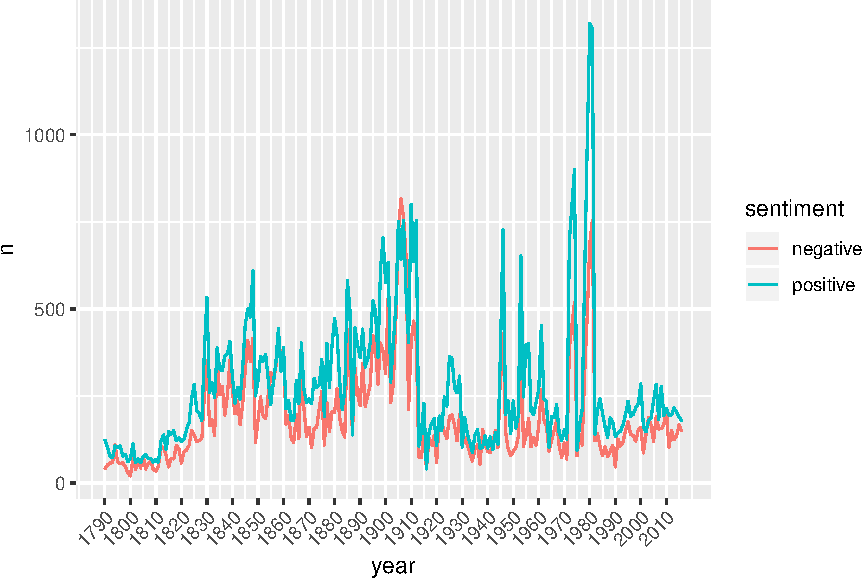
\includegraphics{R-text-analysis_files/figure-latex/sentiment-plot-1.pdf}

\bibliography{book.bib,packages.bib}


\end{document}
